%%%%%%%%%%%%%%%%%%%%%%%%%%%%%%%%%%%%%%%%%
% University/School Laboratory Report
% LaTeX Template
% Version 3.1 (25/3/14)
%
% This template has been downloaded from:
% http://www.LaTeXTemplates.com
%
% Original author:
% Linux and Unix Users Group at Virginia Tech Wiki 
% (https://vtluug.org/wiki/Example_LaTeX_chem_lab_report)
%
% License:
% CC BY-NC-SA 3.0 (http://creativecommons.org/licenses/by-nc-sa/3.0/)
%
%%%%%%%%%%%%%%%%%%%%%%%%%%%%%%%%%%%%%%%%%

%----------------------------------------------------------------------------------------
%	PACKAGES AND DOCUMENT CONFIGURATIONS
%----------------------------------------------------------------------------------------

\documentclass{article}

\usepackage[margin=1in]{geometry}
%\usepackage[version=3]{mhchem} % Package for chemical equation typesetting
%\usepackage{siunitx} % Provides the \SI{}{} and \si{} command for typesetting SI units
\usepackage{graphicx} % Required for the inclusion of images
\usepackage{natbib} % Required to change bibliography style to APA
\usepackage{amsmath} % Required for some math elements 
\usepackage{amssymb}
\usepackage{color}

\def\deriv#1#2{\frac{d #1}{d #2}}
\def\pp#1#2{\frac{\partial #1}{\partial #2}}
\newcommand{\pder}[2][]{\frac{\partial#1}{\partial#2}}
\newcommand{\sder}[2][]{\frac{\partial^{2}#1}{\partial#2^{2}}}

\usepackage{parskip}
\setlength\parindent{45pt} % Removes all indentation from paragraphs

\renewcommand{\labelenumi}{\alph{enumi}.} % Make numbering in the enumerate environment by letter rather than number (e.g. section 6)

%\usepackage{times} % Uncomment to use the Times New Roman font

%----------------------------------------------------------------------------------------
%	DOCUMENT INFORMATION
%----------------------------------------------------------------------------------------

\title{Simulation of Moving Boundaries: Immersed Boundary and Arbitrary Lagrangian-Eulerian Methods} % Title

\author{A. Cody \textsc{Nunno} and Bruce A. \textsc{Perry}} % Author name

\date{\today} % Date for the report

\begin{document}

\maketitle % Insert the title, author and date


% If you wish to include an abstract, uncomment the lines below
\begin{abstract}
In the field of computational fluid dynamics (CFD), most algorithms are developed for use in reference frames where the system boundaries are stationary.  Often, however, moving geometries, such as that of a cylindrical piston, must be considered in order to make predictions regarding real systems.  With that in mind, a set of numerical experiments will be performed on a 2D piston geometry with an advancing, receding, or reciprocating boundary.  To address the changing computational domain, two meshing methods will be implemented and compared: the Arbitrary Lagrangian-Eulerian (ALE) method and the Immersed Boundary (IB) method.  ALE uses a moving grid to maintain accuracy and resolution as the geometry of a system changes.  The IB method uses a stationary mesh but requires the addition of a source term to the governing equations to enforce the boundary conditions when the boundary does not align with the mesh. The advantages and disadvantages of the two methods with regards to simplicity, cost, stability, and accuracy will be compared.
\end{abstract}

%----------------------------------------------------------------------------------------
%	SECTION 1
%----------------------------------------------------------------------------------------

\section{Introduction}

Moving boundaries are often an unavoidable challenge in examining real problems in fluid mechanics.  While for many applications of fluid dynamics involve problems with consistent or stationary boundaries, such as boundary layers or pipe flow, still others require movement of the domain boundaries. In particular, when there is relative motion between different parts of the boundary of the fluid domain, it is impossible to adopt a reference frame where all boundaries are stationary. This will be the case whenever the size or shape of the domain changes in time.  Modern airplane wings shift the shape of the wing to have more advantageous properties for takeoff, flight, or landing, which necessitates a change in boundary conditions for the flow around the craft.  In an internal combustion engine, the pistons move up and down, changing the size and shape of the volume of interest. Other types of flows which involve moving boundaries include flow through blood vessels, wind turbine and propeller flows, and free surface flows. 

The scenarios described above are very difficult to simulate using CFD with conventional boundary conditions.  To this end, other methods have been developed to provide the capability to simulate the fluid flow in these cases. In particular, two methods that have been widely utilized are the Arbitrary Lagrangian-Eulerian (ALE) method and the Immersed Boundary (IB) method. In the former method, a moving grid which adjusts to deforming boundaries of the domain is used \cite{hirt74}. In the latter, a stationary grid is used but additional forcing terms must be added to the equations near the boundaries to account for the boundary movement \cite{peskin1972,mittal2005}. In this work, the background and mathematical formulations for these two methods are discussed, then the implmentation of each method into a Fortran compressible solver is described. The two methods are applied to the canonical 2D piston problem. This geometry has practical significance as a simplified reprsentation of a cylinder of an internal combusion engine. 

 
%----------------------------------------------------------------------------------------
%	SECTION 2
%----------------------------------------------------------------------------------------

\section{Background}

\subsection{ALE}

The first method to be discussed in this work is the Arbitrary Lagrangian-Eulerian (ALE) method, which uses a moving grid to accomplish the change in the control volume of interest.  In most fluid dynamics textbooks, fluids are typically examined in two different frames: Eulerian, which examines the flow by focusing on a fixed space as fluid passes through, and Lagrangian, which follows the flow through space as it moves.  Typically, CFD solves its given problem on an Eulerian grid; this simplifies the method of solution by maintaining a consistent grid, since, especially in flows which are turbulent, or would otherwise require a grid with irregular remeshing.  These two frames are typically related to one another through the material derivative, given by:
\begin{equation}
  \frac{DF}{Dt} = \deriv{F}{t} + u \cdot \nabla F
\end{equation}
where F is merely some function in the domain.  This allows us to relate any quantity in the Eulerian frame with a kinematical description linked to the moving particle.  

A similar technique can be applied to a moving grid.  There is no particular reason that the moving frame must be attached to the particle, except that it is a useful descriptor.  In a CFD simulation, the grid is also a convenient frame; however, the grid is typically also unmoving.  In ALE, there is propagation of the grid according to the boundary conditions of the problem, which gives meaning to the idea of tracking the grid.  In this frame, we can define a velocity which is relative to the grid:
\begin{equation}
  c = u - \hat{u}
\end{equation}
where $\hat{u}$ is the propagation velocity of the grid.  This term, along with the same logic which lead us to the material derivative, allows us to write an expression for the material derivative using quantities in the grid reference frame~\cite{sarrate01}:
\begin{equation}
  \frac{DF}{Dt} = \frac{\eth F}{\eth t} + c \cdot \nabla F
\end{equation}
where $\frac{\eth F}{\eth t}$ is the derivative in the frame of the grid.  It is essentially the same, but now the material derivative is taken in the frame of the moving grid.  This substitution is required in the equations of motion for the Eulerian $\deriv{F}{t}$ so as to avoid needing to perform inaccurate operations to advance the simulation in time.  In our three governing equations:
\begin{equation}
  \frac{\eth \rho}{\eth t} + c_j \pp{\rho}{x_j} + \rho \pp{u_j}{x_j}
\end{equation}
\begin{equation}
  \frac{\eth \rho u_i}{\eth t} + c_j \pp{\rho u_i}{x_j} + (\rho u_i)\pp{u_j}{x_j} = - \pp{p}{x_i} + \pp{\tau_{ij}}{x_j}
\end{equation}
\begin{equation}
  \frac{\eth \rho e_t}{\eth t} + c_j \pp{\rho e_t}{x_j} + (\rho e_t)\pp{u_j}{x_j} = - \pp{p u_j}{x_j} + \pp{\tau_{ij} u_j}{x_j}  - \pp{q_j}{x_j}
\end{equation}

ALE is a very popular method for fluid dynamics simulations which involve a shifting grid, especially those which involve fluid interfaces.  Fluid structure interactions are a primary use for the ALE method.  Schemes similar to ALE, though not necessarily called such, have been in use for fluid structure interactions since the 1960's~\cite{noh63,trulio66}, but the first implementation of a method called Arbitrary Lagrangian-Eulerian was introduced specifically for problems with flexible boundaries, such as a heart valve~\cite{hirt74}.  In many of the papers regarding fluid-solid interactions, the finite element technique has been used~\cite{hron06,letallec01,souli00}, presumably due to the frequent simulation of the solid in addition to the fluid, where the finite element technique is more appropriate than others.  Common configurations in such cases include channel flow with moving walls, such as one might see in a biological flow~\cite{hron06}, or flow over a body, deformable or otherwise~\cite{farhat05}.  Boundary conditions for fluid-solid interfaces are usually typical no-slip surfaces, where the displacement and velocity of the interface are the same, with one slight addition.  The simulation of the body and fluid requires some knowledge about their interface and the momentum transfer between them; therefore, we require that the stress across the boundary also be the same to enforce the boundary conditions.

Another problem of interest in ALE is free surface flows.  These types of problems are largely between a liquid and a gas, applied to wave propagation problems~\cite{braess00,lo04,nithiarasu05}.  The interface between the two fluids can be represented through the same techniques as the solid-fluid interaction.  In most cases, a finite element program is still used to solve the discretized equations.  The most challenging element unique to a free surface problem is obviously the propagation of the free surface wave front.  To solve this problem, one of two approaches is usually followed.  The first requires solving a kinematic equation for the surface, of the form:
\begin{equation}
  \pp{z}{t} + (v\cdot \nabla)z = 0
\end{equation}
The second method merely requires that the velocity across the interface is zero, which allows the surface to propagate as normal~\cite{sarrate01}.

Perhaps the greatest uncertainty which pertains to the ALE method is the mesh propagation.  If one has a cyclical or otherwise predictable moving boundary, the mesh propagation is fairly simple as it can be decided upon as some function of the boundary movement, but the problem becomes harder is the motion is not known \emph{a priori}.  From there, one must choose whether or not one wishes to retain the same mesh or occasionally remesh.  Maintaining the same mesh, called regularization~\cite{sarrate01}, uses the propagation of the boundary to determine how the boundary moves as well.  The movement of the boundary must be determined, then the mesh movement can be determined through a set of potential-like equations which can be decribed, at least generally, \emph{a priori}.  An adaptive mesh can also be used to describe these more complicated meshes, wherein the mesh seeks to move points towards areas of strong gradient while also simultaneously trying to spread error out evenly across the entire domain~\cite{sarrate01}.  This technique has been used effectively in flows, and is especially useful when anisotropy is important.

With any method there are both adavantages and disadvantages.  The ALE method's primary usefulness is its ability to study moving grids, which can be the most effective method for certain types of problems.  It has significant advantages over purely Eulerian grids in that it is very easy to track the solid interface boundary, and by moving the mesh separate from the fluid, it can avoid the twisting typically associated with a Lagrangian mesh.  Additionally, the moving grid formulation is particularly applicable for moving objects where the solid is also simulated, as the interfaces can be done using the same moving grid.  However, as always, there are drawbacks.  As stated previously, the grid propagation is not easy to determine without \emph{a priori} knowledge unless remeshing is to be used; the first can result in mesh entangling, but the second is computationally expensive.   As will be discussed in the Implementation section, the form of the equations is inherently non-conservative for momentum, and the stability properties are irregular and hard to determine due to the ever changing grid size~\cite{hirt74}.  Additionally, moving a grid through space without fixed boundaries can result in mass non-conservation if properties are kept at cell centers instead of cell faces~\cite{ferziger12}.  This is more an issue with finite volume methods than the finite differences used in this work, but is worth mentioning.

\subsection{Immersed Boundary}

Immersed boundary methods refer to any of a class of methods in which a stationary, regular (usually cartesian) grid is overlaid on a domain with moving or irregularly shaped boundaries. hile IB-like methods \cite{scardovelli1999direct} can be applied to fluid-fluids interfaces, because the case to be studied here involves a moving solid wall, the immersed boundaries will subsequently be assumed to be solid walls for simplcity. These methods were originally developed to study flow in complex but stationary geometries, and the first application was to the study of flow through a heart valve by Peskin in 1972.\cite{peskin1972} The key distinguishing feature of an IB method is that the solid boundary does not exactly coincide with the grid locations of the flow variables. It can be seen that for the case of a continuously moving boundary and a stationary grid, the boundary location must not always coincide with the grid points, and therefore IB methods are relevant. In general, the main advantage of this approach, whether for complex geometries, moving geometries, or both, is that a cartesian grid and straightforward numerical methods, such as finite difference approaches, can be used. The disadvantage is that because the boundaries and grid are not aligned, the effects of the boundaries on the flow must be modeled rather than being directly accounted for. This is illustrated in Figure \ref{fig:ibpic}.

\begin{figure}
  \centering
 %\begin{overpic}
    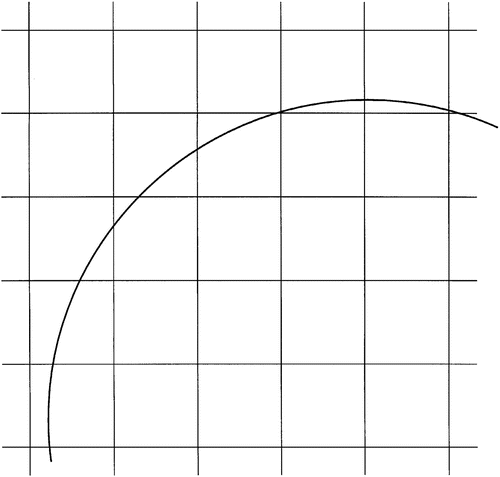
\includegraphics[width = 2in]{ibpic}
    \put (2,98) {$\Gamma_b$}
    \put (-125,114) {$\Omega_f$}
    \put (-56,39) {$\Omega_b$}
  %\end{overpic}
  \caption{\label{fig:ibpic} Schematic of a curved boundary ($\Gamma_b$) with a structure grid overlaid. The fluid ($\Omega_f$) and solid ($\Omega_b$) domains are labeled. Adapted from \cite{scardovelli1999direct} }
\end{figure}

There are two main approaches to implementation of the immersed boundary method, continuous and discrete forcing, which differ in the way that a forcing term is added to account for the boundary \cite{mittal2005}. In general, the governing equations for a fluid mechanics simulation can be expressed as
\begin{equation}
\mathcal{L}(\bar{U}) = 0 \hspace{12pt} \rm{in} \hspace{12pt}  \Omega_f,
\end{equation}
with boundary conditions
\begin{equation}
\bar{U} = \bar{U}_\Gamma \hspace{12pt} \rm{on} \hspace{12pt}  \Gamma_b,
\end{equation}
where $\bar{U}$ is a vector of the flow variables (velocities, density, pressure, and temperature/internal energy) and $\mathcal{L}$ is an operator defined by the continuity, momentum, and energy equations. In the continuous forcing approach, a smooth forcing function ($\bar{f}_b$ is added to the continuous equations, which must be considered on the full domain because the forcing function is smooth and has nonzero values within the fluid and solid near the boundary:
\begin{equation}
\mathcal{L}(\bar{U}) = \bar{f}_b \hspace{12pt} \rm{in} \hspace{12pt}  \Omega_f + \Omega_b.
\end{equation}
The disadvantage of this approach is that a diffuse forcing function is required to ensure that the effect of the boundary is felt at the nearby grid cells, but this corresponds to a \lq fuzzy\rq\ boundary. In contrast, the discrete forcing approach involves first discretizing the governing equations, then adding a forcing term only at the boundary, resulting in the modified set of equations:
\begin{equation}
\mathcal{L}_d(\bar{U}) = 0 \hspace{12pt} \rm{in} \hspace{12pt}  \Omega_f.
\end{equation}
\begin{equation}
\mathcal{L}'_d(\bar{U}) = \bar{r} \hspace{12pt} \rm{near} \hspace{12pt}  \Gamma_b.
\end{equation}
where $\mathcal{L}_d$ is the discretized operator, $\mathcal{L}'_d$ is the modified operator that applies near the boundaries, and $\bar{r}$ is a vector of effective forcing terms based on the known conditions at the boundary. Because forcing is added after discretization, it is possible to obtain an effectively sharp fluid-solid interface.

Because the system to be examined involves sharp fluid-solid boundaries, the discrete forcing approach is used in this work. Based on the discussion above, the use of the immersed boundary method does not affect the solution procedure away from the boundaries for finite difference discretizations. However, near the boundaries the modified discretized spatial operator will need to account for two types of nodes differently: ghost nodes and freshly cleared nodes. As illustrated in Figure \ref{fig:ghost}, ghost nodes are nodes that lie within the solid domain but are adjacent to one or more nodes in the fluid domain. Values of flow variables at these nodes must be specified in order to use finite difference methods to calculate derivatives at the adjacent nodes within the fluid domain. The values are specified such that interpolation between the ghost node (G) and the adjacent fluid nodes (F1,F2,F3) to the point B on the boundary results in a value that satisfies the boundary condition at B, which is the normal intercept from the ghost node to the immersed boundary. This interpolation can be expressed as:
\begin{equation}
\phi_B = \omega_G \phi_G + \omega_{F1} \phi_{F1} + \omega_{F2} \phi_{F2}  + \omega_{F3} \phi_{F3}
\end{equation}
and therefore
\begin{equation}
\label{eqn:ghostnode}
\phi_G = \frac{\phi_B - \omega_{F1} \phi_{F1} - \omega_{F2} \phi_{F2}  - \omega_{F3} \phi_{F3}}{\omega_G}.
\end{equation}
where $\omega_i$ are geometry-dependent interpolation weightings and $\phi$ is any flow variable.
The freshly cleared nodes are nodes which were within the solid boundary at timestep $n-1$ but at timestep $n$ are now in the fluid domain due to the movement of the boundary. The values of flow variables at these nodes are not defined at timestep $n$ and must be determined by interpolation between the adjacent fluid nodes and the boundary. 

\begin{figure}
  \centering
    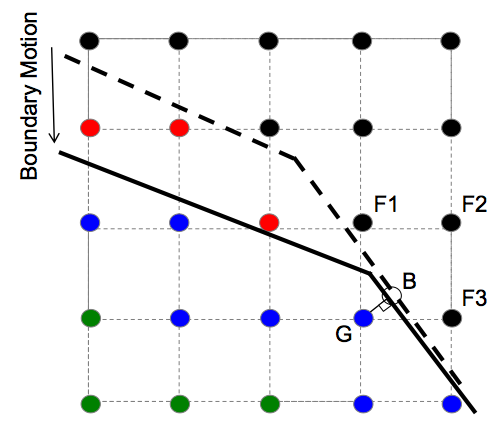
\includegraphics[width = 2in]{ghost}
  \caption{\label{fig:ghost} Schematic for finite difference spatial discretization with a moving immersed boundary, showing nodes in the fluid domain (black), nodes in the solid domain (green), ghost nodes (blue), and freshly cleared nodes (red). }
\end{figure}

Because the IB method was originally developed for flows with geometrically complex but stationary boundaries, but can be directly extended to flows with moving boundaries, it is particularly well suited to flows with boundaries that are both complex and moving. In fact, the IB method can be used to simulate arbitrary geometries with arbitrary motion. For example, the IB method has been used to simulate flow within a model internal combustion engine including the valves, \cite{fadlun2000combined} and the flow generated by a hummingbird's flapping wings \cite{song2014three}. These are cases for which prescribing the motion of the grid in an ALE approach would have been challenging due to the geometrical complexity. Another advantage of the IB method is that it does not affect the numerical method or equations being solved in the bulk of the fluid as compared to a flow with stationary boundaries. It is therefore simpler to extend adapt existing codes using the IB method. Furthermore, because the numerical methods are unaffected, the stability, conservation, and accuracy properties of the simulation can be controlled by selecting appropriate numerical methods and discretization schemes.  

The disadvantages of the IB method relate mainly to the need to include the extra nodes which are covered by the solid boundary. Although in most IB implementations it is not necessary to iterate forward in time at the covered nodes, and therefore these nodes contribute minimally to the total number of operations that must be performed, including these nodes does significantly increase the memory requirement. An additional effect is that because the boundaries move relative to the grid, if higher resolution is desired near the boundaries, more grid points must be added throughout the domain, or at least to any region which the boundary may plausibly move to. A disadvantage is that calculation of the forcing function or geometry-dependent interpolation coefficients for the immersed boundary method can be challenging and expensive if the geometry is complex, or moving such that the coefficients must be recalculated at every timestep. 

%----------------------------------------------------------------------------------------
%	SECTION 3
%----------------------------------------------------------------------------------------

\section{Method of Solution}
Due to significant differences in the structure of the code required for the ALE and IB approaches, the two were implemented in separate, but similar Fortran programs. The moving piston test case to be considered can involve significant compression or expansion as well as motion at non-negligible Mach numbers, so compressible flow solvers were developed. An additional advantage of using a compressible solver is that its implementation for the ALE and IB methods is more straightforward than pressure-Poisson equation based incompressible solvers. For example, because covered nodes in the IB method are ignored, the dimension of linear system that would need to be solved to solve the pressure-Poisson equation would vary from timestep to timestep. 

For both moving boundary methods, the explicit Euler approach is used for temporal discretization and second-order central differencing is used for spatial discretization. The central spatial scheme was selected because to ensure stability biased schemes must be biased in the upwind direction, and determining the upwind direction for the moving ALE grid while also accounting for acoustic wave propagation would not be simple. Iteration in time occurs in two steps: first, heat flux ($q$) and shear stress ($\tau$) values are calculated at the midpoints between the nodes and, second, all first derivatives are calculated and the solution is advanced by one timestep. Thus, a staggered grid arrangement is used where $P$, $\rho$, $T$, $u$, $v$, and the relevant density-weighted variables are stored at nodes and the stresses and fluxes are stored at the midpoints between nodes, as illustrated in Figure \ref{fig:grid}. This approach is essentially identical to using a standard second-order central scheme to calculate the second derivatives in the stress and flux terms in the equations. 

The 2D piston geometry to be considered is bounded on all sides by walls. Therefore, the velocity boundary conditions are given by enforcing no slip on the walls. The walls are assumed to be held constant at the intitial temperature of the system. However, an additional condition on density or pressure is required to fully specify the state at the boundary. Navier-Stokes Characteristic Boundary Conditions \cite{} were considered, but the simulations could not be made stable when using these boundary conditions. Therefore, a simpler pressure extrapolation boundary condition was used, basing the pressure at the boundary on the pressure at the adjacent cell and the gradient at the adjacent cell:
\begin{equation}
p^n_{i,B} = p^n_{i,B-1} + (p^n_{i,B-1} - p^n_{i,B-2}),
\end{equation}
where it has been assumed that the grid spacing is uniform and the subscript $B$ refers to the index of the boundary node.

\begin{figure}
\centering
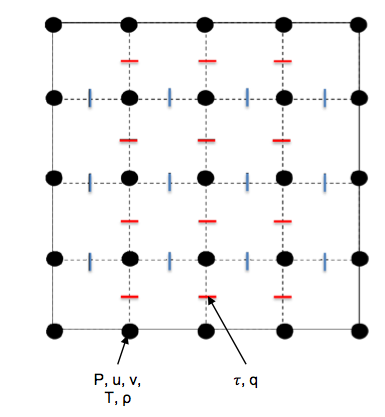
\includegraphics[width=2in]{grid}
\caption{\label{fig:grid} Staggered grid for solution of the compressible flow equations. Velocity and thermodynamic state variables are stored at the nodes, while fluxes and stresses are stored at the midpoints between nodes. Fluxes in the $x$-direction are stored at the $x$-direction midpoints (blue lines) and $y$ fluxes are stored at $y$ midpoints (red lines). }
  \end{figure}	
    

\subsection{ALE}

For the ALE solver, the governing equations are discretized and solved in dimensional form.  To illustrate the method of solution, the continuity, momentum, and energy equations, as discretized, are repeated below:

\begin{equation}
  \begin{aligned}
    \frac{\rho^{n+1}_{i,j} - \rho^{n}_{i,j}}{\Delta t} = - u^{n}_{i,j} \frac{\rho^{n}_{i+1,j}-\rho^{n}_{i-1,j}}{2\Delta x} - c^{n}_{i,j} \frac{\rho^{n}_{i,j+1}-\rho^{n}_{i,j-1}}{2\Delta y} + \rho^{n}_{i,j} \left(\frac{u^{n}_{i+1,j}-u^{n}_{i-1,j}}{2\Delta x} + \frac{u^{n}_{i,j+1}-u^{n}_{i,j-1}}{2\Delta y}\right)
  \end{aligned}
\end{equation}
\begin{equation}
  \begin{aligned}
    \frac{(\rho u)^{n+1}_{i,j} - (\rho u)^{n}_{i,j}}{\Delta t} &= - u^{n}_{i,j} \frac{(\rho u)^{n}_{i+1,j}-(\rho u)^{n}_{i-1,j}}{2\Delta x} - c^{n}_{i,j} \frac{(\rho u)^{n}_{i,j+1}-(\rho u)^{n}_{i,j-1}}{2\Delta y} \\
    &+ (\rho u)^{n}_{i,j} \left(\frac{u^{n}_{i+1,j}-u^{n}_{i-1,j}}{2\Delta x} + \frac{v^{n}_{i,j+1}-v^{n}_{i,j-1}}{2\Delta y}\right) - \frac{p^{n}_{i+1,j} - p^{n}_{i-1,j}}{2\Delta x} \\
    &+ \frac{(\tau_{xx})^{n}_{i+1/2,j} - (\tau_{xx})^{n}_{i-1/2,j}}{\Delta x} + \frac{(\tau_{yx})^{n}_{i,j+1/2} - (\tau_{yx})^{n}_{i,j-1/2}}{\Delta y}
  \end{aligned}
\end{equation}
\begin{equation}
  \begin{aligned}
    \frac{(\rho v)^{n+1}_{i,j} - (\rho v)^{n}_{i,j}}{\Delta t} &= - u^{n}_{i,j} \frac{(\rho v)^{n}_{i+1,j}-(\rho v)^{n}_{i-1,j}}{2\Delta x} - c^{n}_{i,j} \frac{(\rho v)^{n}_{i,j+1}-(\rho v)^{n}_{i,j-1}}{2\Delta y} \\
    &+ (\rho v)^{n}_{i,j} \left(\frac{u^{n}_{i+1,j}-u^{n}_{i-1,j}}{2\Delta x} + \frac{v^{n}_{i,j+1}-v^{n}_{i,j-1}}{2\Delta y}\right) - \frac{p^{n}_{i,j+1} - p^{n}_{i,j-1}}{2\Delta y} \\
    &+ \frac{(\tau_{xy})^{n}_{i+1/2,j} - (\tau_{xy})^{n}_{i-1/2,j}}{\Delta x} + \frac{(\tau_{yy})^{n}_{i,j+1/2} - (\tau_{yy})^{n}_{i,j-1/2}}{\Delta y}
  \end{aligned}
\end{equation}
\begin{equation}
  \begin{aligned}
    \frac{(\rho e_t)^{n+1}_{i,j} - (\rho e_t)^{n}_{i,j}}{\Delta t} &= - u^{n}_{i,j} \frac{(\rho e_t)^{n}_{i+1,j}-(\rho e_t)^{n}_{i-1,j}}{2\Delta x} - c^{n}_{i,j}\frac{(\rho e_t)^{n}_{i,j+1}-(\rho e_t)^{n}_{i,j-1}}{2\Delta y} \\
    &+ (\rho e_t)^{n}_{i,j} \left(\frac{u^{n}_{i+1,j}-u^{n}_{i-1,j}}{2\Delta x} + \frac{v^{n}_{i,j+1}-v^{n}_{i,j-1}}{2\Delta y}\right) - \frac{p^{n}_{i+1,j}u^{n}_{i+1,j} - p^{n}_{i-1,j} u^{n}_{i-1,j}}{2\Delta x} \\
    &- \frac{p^{n}_{i,j+1} v^{n}_{i,j-1} - p^{n}_{i,j-1} v^{n}_{i,j-1}}{2\Delta y} + \frac{u^{n}_{i+1/2,j}(\tau_{xx})^{n}_{i+1/2,j} - u^{n}_{i-1/2,j} (\tau_{xx})^{n}_{i-1/2,j}}{\Delta x} \\
    &+ \frac{v^{n}_{i,j+1/2} (\tau_{yx})^{n}_{i,j+1/2} - v^{n}_{i,j-1/2} (\tau_{yx})^{n}_{i,j-1/2}}{\Delta y} + \frac{u^{n}_{i+1/2,j} (\tau_{xy})^{n}_{i+1/2,j} - u^{n}_{i-1/2,j}(\tau_{xy})^{n}_{i-1/2,j}}{\Delta x}  \\
    &+ \frac{v^{n}_{i,j+1/2} (\tau_{yy})^{n}_{i,j+1/2} - v^{n}_{i,j-1/2} (\tau_{yy})^{n}_{i,j-1/2}}{\Delta y} - \frac{(q_x)^{n}_{i+1/2,j} - (q_x)^{n}_{i-1/2,j}}{\Delta x} - \frac{(q_y)^{n}_{i+1/2,j} - (q_y)^{n}_{i-1/2,j}}{\Delta y}
  \end{aligned}
\end{equation}
The values of density weighted quantities, $\rho$, $\rho u$, $\rho v$, and $\rho e_t$, can be found using these equations, and then the values of the corresponding primitive variables ($u$ and $v$) are determined at the end of the timestep by dividing by $\rho$.  Other variables, such as $p$ and $T$, can be found using the definition of energy,
\begin{equation}
  \rho e_t = \frac{1}{\gamma -1} p + \frac{1}{2} \rho (u^2 + v^2)
\end{equation}
\begin{equation}
  p = \rho R T
\end{equation}
The primary difference between this implementation and the implementation used for the IB method is that the equations are dimensional so as to make the introduction of the grid velocity conceptually simpler.

\subsection{Immersed Boundary}

For the immersed boundary method, the governing equations are discretized in a manner similar to that used in the ALE method, although clearly the grid propagation velocity need not be considered for the stationary IB grid. However, the governing equations are non-dimensionalized to better elucidate the effects of the flow conditions on the result in terms of non-dimensional parameters. The resulting continuous equations are:
%
\begin{equation}
\label{continuity-non}
\Omega_r \pder[\rho]{t} +  \pder[\rho u_j]{x_j} = 0
\end{equation}
%
\begin{equation}
\label{momentum-non}
\Omega_r \pder[\rho u_i]{t^*} + \pder[\rho u_j u_i]{x_j} = -\frac{1}{\gamma \textrm{Ma}^2}\pder[p]{x_i} + \frac{1}{\textrm{Re}} \pder[\tau_{ij}]{x_j}
\end{equation}
%
\begin{equation}
\label{temp-non}
\Omega_r \pder[\rho e_t]{t} + \pder[\rho u_j e_t]{x_j} = 
\frac{\gamma}{PrRe}\sder[T]{x_j} - (\gamma -1) \pder[p u_j]{x_j}
- (\gamma -1)\gamma \frac{\textrm{Ma}^2}{\textrm{Re}} \pder{x_j} \left( \tau_{ij}u_i  \right)
\end{equation}
%
\begin{equation}
\label{idg-non}
p = \rho T.
\end{equation}
%
where all variables are non-dimensional and subscripts $i$ and $j$ are direction indices. The non-dimensional parameters in the equation are:
\begin{equation}
\begin{aligned}
\textrm{Re} =& \ U_W L / \nu \\
\gamma =& c_p/c_v = 1.4\\
\textrm{Ma}_r =&\ U_W/a_r \\
\textrm{Pr} =&\ \rho c_p \nu / \lambda = 0.7 \\
\Omega =& \omega L / U
\end{aligned}
\end{equation}
where $U_W$ is a characteristic velocity, $L$ is a characteristic length scale, $\omega$ is a characteristic frequency, and $a_r$ is the speed of sound at reference conditions. 

The governing equations are solved in conservative form to ensure that the numerical scheme is primary conservative. In discretized form,  the continuity and $x$-momentum equations become:
\begin{equation}
\Omega \frac{\rho_{i,j}^{n+1} - \rho_{i,j}^n}{\Delta t} = \frac{(\rho u)_{i+1,j}^{n} - (\rho u)_{i-1,j}^n}{2 \Delta x} + \frac{(\rho v)_{i,j+1}^{n} - (\rho v)_{i,j-1}^n}{2 \Delta y}
\end{equation}
\begin{equation}
\begin{aligned}
\Omega \frac{(\rho u)_{i,j}^{n+1} - (\rho u)_{i,j}^n}{\Delta t} 
&= - \frac{(\rho u u)_{i+1,j}^{n} - (\rho u u)_{i-1,j}^n}{2 \Delta x} 
- \frac{(\rho u v)_{i,j+1}^{n} - (\rho u v)_{i,j-1}^n}{2 \Delta y}  \\
&+ \frac{1}{\rm{Re}}\frac{(\tau_{xx})^n_{i+\frac{1}{2},j} -  (\tau_{xx})^n_{i-\frac{1}{2},j}}{\Delta x}
+ \frac{1}{\rm{Re}}
\frac{(\tau_{yx})^n_{i,j+\frac{1}{2}} -  (\tau_{yx})^n_{i,j-\frac{1}{2}}}{\Delta y}
- \frac{1}{\gamma \rm{Ma}^2} \frac{p^n_{i+1,j} - p^n{i-1,j}}{2 \Delta x}
\end{aligned}
\end{equation}
where again all flow variables are non-dimensional. The $y$-momentum and energy equations have analogous forms. The solution procedure is similar to that for the ALE method, in that the density weighted variables are determined using the above equations, then primitive variables are calculated by dividing by density and using the equation of state. 

The above discretized equations hold at all locations within the fluid domain. However, it is also necessary to solve for the ghost and freshly cleared nodes at each timestep. The ghost nodes are calculated using the method shown in Equation \ref{eqn:ghostnode}. However, because in the 2D piston geometry to be considered the piston is oriented parallel to one of the directions of the grid, the interpolation is only needed in one direction. Therefore, the value of any flow variable $\phi^n$ at a ghost cell can be calculated:
\begin{equation}
\phi^n_{i,G} = \frac{\phi_{i,B}^n - \phi^n_{i,G-1} (1- \alpha)}{\alpha}
\end {equation} 
where the subscript $G$ is the $y$-index of the ghost node, $\phi_{i,B}^n$ is the value of the flow variable at the boundary, and $\alpha$ is an interpolation weight calculated through:
\begin{equation}
\alpha = \frac{y_B - y_{G-1}}{y_G - y_{G-1}}.
\end{equation} 
If there are any freshly cleared nodes, the values at the ghost nodes are determined using the boundary conditions and the first non-freshly cleared node in the fluid domain. Then, the values at the freshly cleared nodes are calculated by interpolation between the boundary and the first non-freshly cleared node in the fluid domain.

%%%%%%%%%%%%%%%%%%%%%%%%%%%%%%%%%%%%%%%
%
%                                              Verification
%
%%%%%%%%%%%%%%%%%%%%%%%%%%%%%%%%%%%%%%%%

\section{Verification}

\subsection{ALE}

As we are continuing to use second order central difference and explicit Euler, convergence should be second order in space and first order in time. The convergence of the solvers in both time and space can be determined without knowing the analytical solution.\cite{macart}. For a scheme of order $n$ the psuedo-error, $\epsilon$, follows the relation:
\begin{equation}
\centering
\epsilon = |\tilde{u}_{\Delta t} - \tilde{u}_{\Delta t/2}| = |\kappa - 2^{-n}| (\Delta t)^n = \kappa' (\Delta t)^n ,
\label{eqn:error2}
\end{equation}
from which the order $n$ can be determined without knowing $u_e$. In particular, the slope of a log-log plot of $\epsilon$ vs $\Delta t$ gives the order of temporal convergence. Note that if the above equation holds for all points, so a plot of the sum of the errors at all points will have a similar property. Also, an analogous expression could be derived for the error due to spatial discretization to find the order of the spatial discretization schemes.  The anticipated time convergence is achieved, as can be seen in Figure~\ref{fig:timeconvALE}.  However, as seen in Figure~\ref{fig:spaceconvALE}, the accuracy spatially is less certain.  Some properties certainly appear to be second order convergent (the velocities), but the quantities which are not explicitly solved for (pressure and temperature) have convergence which is highly irregular and does not match a discernable pattern.  It could be that there is a bug in the energy equation, or perhaps even it is an effect of the ALE method, although the literature has not suggested the latter conclusion.

\begin{figure}
    \centering
    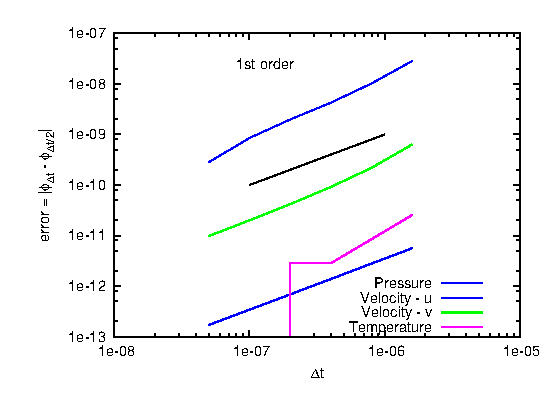
\includegraphics[width=0.6\textwidth]{timeconvALE.eps}         
    \caption{Time convergence for ALE.}
    \label{fig:timeconvALE}
  \end{figure}
\begin{figure}
    \centering
    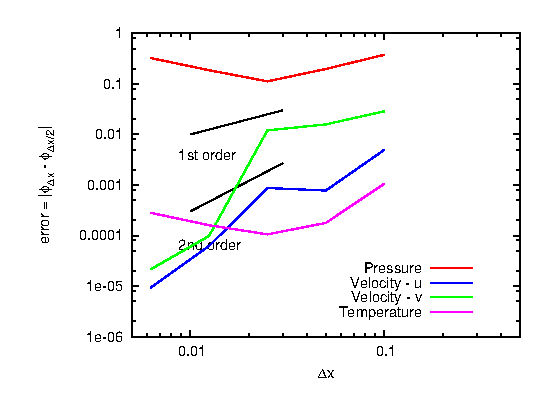
\includegraphics[width=0.6\textwidth]{spaceconvALE.eps}         
    \caption{Spatial convergence for ALE.}
    \label{fig:spaceconvALE}
  \end{figure}
  
Because of the shrinking and expanding grid size, it is impossible to get an exact timestep restriction for ALE.  However, Hirt has previously performed analogous linear stability analysis for ALE~\cite{hirt74}, where the stability criterion is found to be:
\begin{equation}
  \Delta t < \left[ \frac{2(2\mu + \lambda)}{\rho}\left(\frac{1}{\Delta x} + \frac{1}{\Delta y}\right)\right]^{-1}
\end{equation}
where $\lambda$ and $\mu$ are the first and second components of viscosity.  Generally, our methods stability seemed to be rather below that, with strange oscillations forming at factors much lower than indicated here.  Presumably, this is a result of the changing cell size.

\begin{figure}
  \centering
  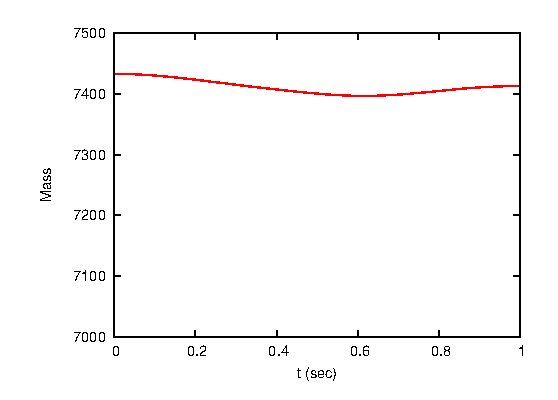
\includegraphics[width=0.6\textwidth]{massconsALE.eps}         
  \caption{Mass conservation for ALE.}
  \label{fig:massconsALE}
\end{figure}
The conservation properties of the ALE solver change fairly significantly over the original solver from the previous project.  This change is necessary, as the change of reference frame requires the separation of the divergence into two components.  It alters the symmetry of the momentum governing equations' summations, which means that they no longer sum to zero over the entire domain.  However, because of the particular problem configuration addressed in this work, neither momentum nor energy conservation can be verified.  Since a moving piston boundary is being considered, work is being done either on or by the system; therefore, the energy and momentum of the system are being directly affected.  We can, however, still establish mass conservation, by summing the densities multiplied by the volume of each cell and the number of cells.  This information is tracked in Figure~\ref{fig:massconsALE}.  It is evident from the image that mass is not quite fully conserved, though the variation is minimal over a full cycle, less than 1\% of the total.  

\subsection{Immersed Boundary}

Because the same discretization schemes were used as in the ALE case, it is again expected that there should be first order convergence in time and second order convergence in space as the time step and grid spacing is reduced, respectively. Again, convergence is checked by plotting the psuedo-error as a function of step size. The temporal and spatial convergence are shown in Figures \ref{fig:timeconvib} and \ref{fig:spaceconvib}. The expected convergences are observed for all variables, indicating that the numerical methods are properly implemented. 

\begin{figure}
    \centering
    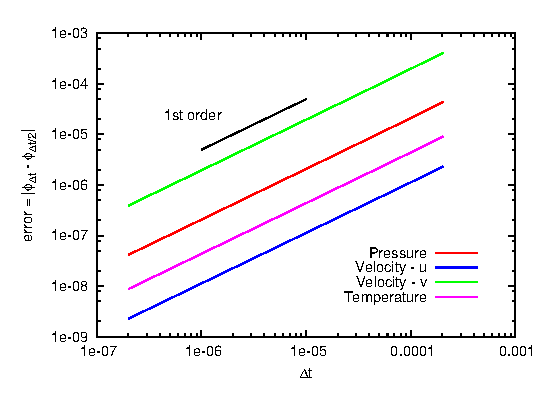
\includegraphics[width=0.6\textwidth]{timeconvib.eps}         
    \caption{Time convergence for the immersed boundary method.}
    \label{fig:timeconvib}
  \end{figure}
\begin{figure}
    \centering
    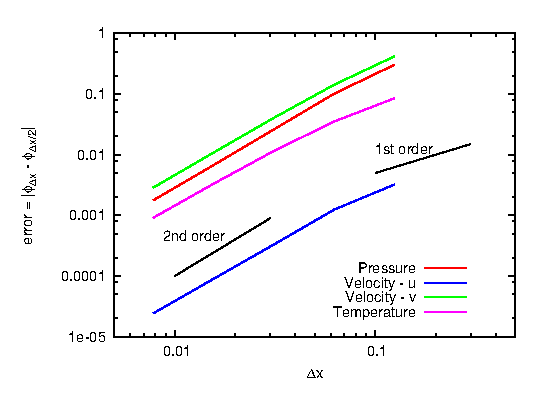
\includegraphics[width=0.6\textwidth]{spaceconvib.eps}         
    \caption{Spatial convergence for the immersed boundary method.}
    \label{fig:spaceconvib}
  \end{figure}

As with the ALE method, conservation of total mass within the system was also verified. The total system mass, calculated by multiplying each node density by its corresponding volume while accounting for the effect of corners, edges, and the immersed boundary on the volume, is plotted as a function of time in Figure \ref{fig:plot-cons-ib}. It can be seen the the total mass decreases slightly for the withdrawing piston, while it increases slightly over time for the advancing piston. In both cases, the total change in mass is very small, less than 1\% of the initial mass. Therefore, this slight non-conservation of mass has minimal impact on the other results. It is thought that change in mass over time is a result of the constant gradient boundary condition used for pressure, particularly at the immersed boundary. 

\begin{figure}
    \centering
    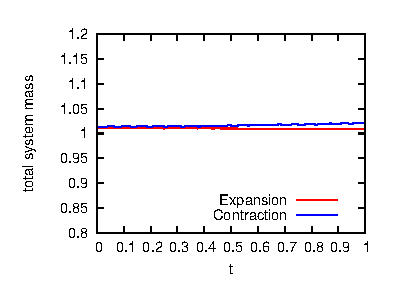
\includegraphics[width=0.6\textwidth]{plot-cons-ib.eps}         
    \caption{Total system mass as a function of time for expanding and contracting piston cases}
    \label{fig:plot-cons-ib}
  \end{figure}


%----------------------------------------------------------------------------------------
%	SECTION 4
%----------------------------------------------------------------------------------------

\section{Application: The Moving Piston}

The great advantage of using both of these methods is their ability to handle moving objects within the flow, or objects which move the flow.  To that end, the test selected to demonstrate these methods is a canonical problem in fluid mechanics that incorporates a moving boundary: the flow incuded by a moving piston.  As considered, the problem is two dimensional, with a fixed width in $x$ and a fixed height in $y$, which are initially equal.  Three types of piston motions are considered: constant velocity impulsive advancement and retraction of the piston, as well as sinusoidal reciprocation. The impulsive start to the piston motion in the constant velocity cases is not physically realistic, butthese simpler cases were used to test to code prior to moving to the oscillatory case. For the latter case, the velocity of the wall is given by 
\begin{equation}
  v_w = \pi \omega A \sin{2 \pi \omega t}
\end{equation}
where A is the amplitude of the oscillations. This can be expressed non-dimensionally as 
\begin{equation}
  v_w^* = \Omega \sin{t^*}.
\end{equation}
For the test cases run here, constant velocity motions were run at the same velocity as the maximum velocity of the oscillatory case.

\begin{figure}
  \centering
  \hspace{12pt} 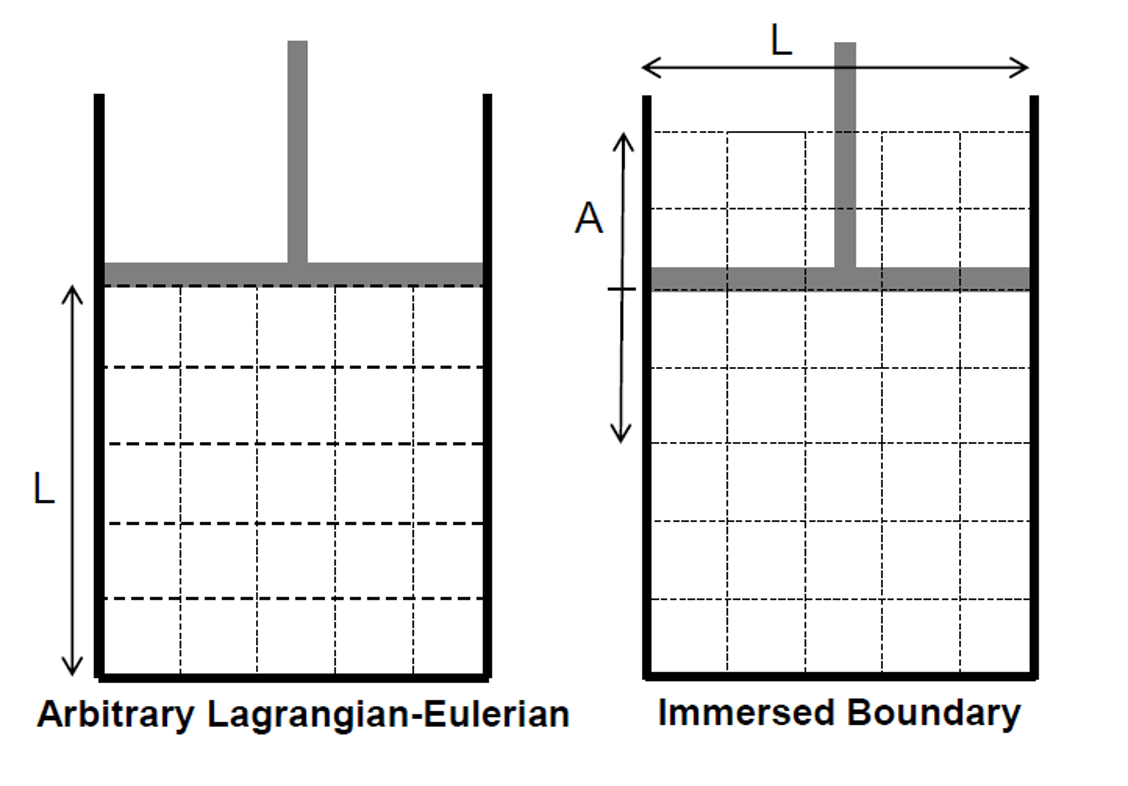
\includegraphics[width=0.5\textwidth]{pistonbef.png}      \\
  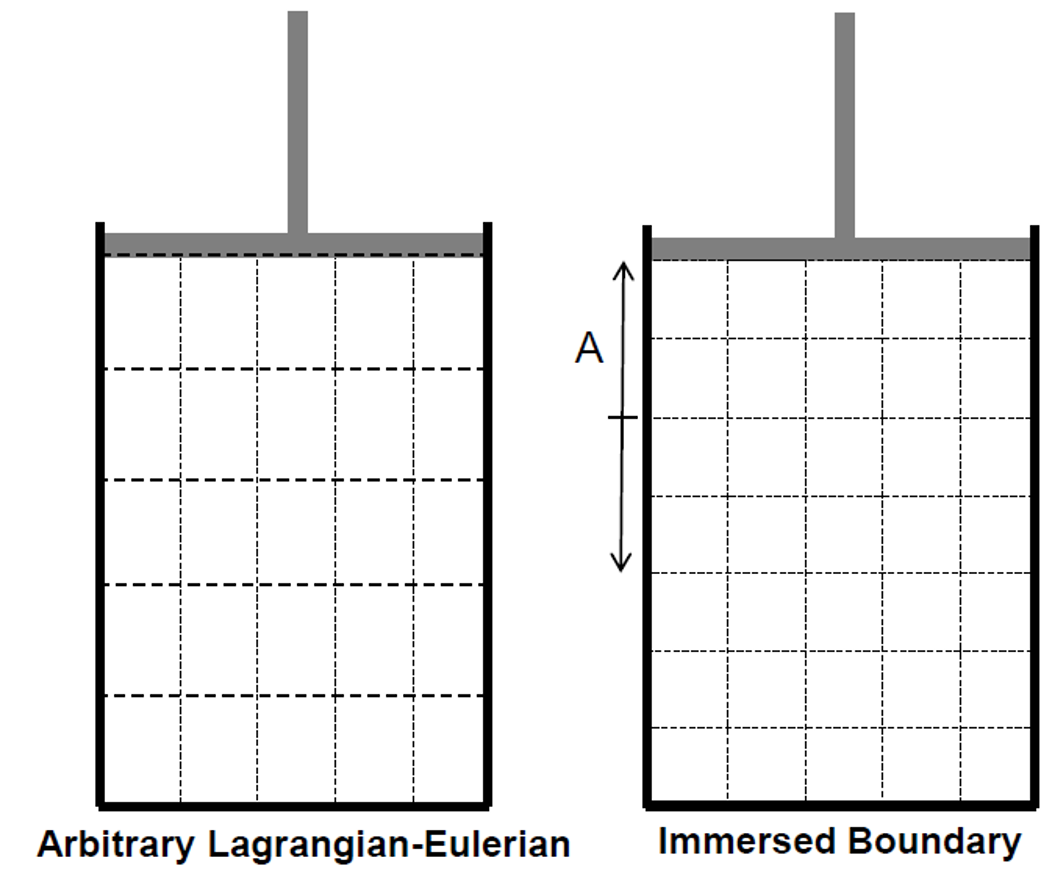
\includegraphics[width=0.46\textwidth]{pistonaft.png}         
  \caption{Piston geometry initially (above) after a full expansion (below), showing grid deformation in the ALE case and covered nodes in the IB case.}
  \label{fig:pistonaft}
\end{figure}


To compare between the two different methods presented, some non-dimensional parameters need to be established to maintain commonality in testing.  The piston Reynolds number, non-dimensional cycle frequency $\omega l/U$, and non-dimesional displacement $A/L$ were all kept approximately constant between the ALE and IB method cases.  Additionally, while the Mach numbers varied between the two methods, for both cases the Mach number was well less than 0.3 and therefore compressibility should have a negligible impact on both. This allows for comparisons between the predictions of each solution method.

\subsection{ALE}

At the conditions of primary testing, the ALE method performed reasonably well.  For testing parameters, some dimensional and dimensionless quantities used as initial conditions are given here.  The box size, L, was 1 m, and the advancement/recession distance was 0.4 m.  Reynolds number was approximately 5, Ma was 0.002, and $\omega L/U$ is approximately 5.  Initial pressure was 100 kPa and temperature was 300 K.  For the constant velocity expansion and contraction cases, the measured quantities behave as expected at long time.  Velocity and pressure as compared to the IB method can be seen in Figures~\ref{fig:constexp} and~\ref{fig:constcomp}.  There were, however, some minor issues initializing the constant withdrawal, as well as the compression.  Initially, the velocity field seemed to oscillate quite rapidly, presumably due to pressure waves initiated by the high jerk impulsive start of the piston.  As the simulation moves through time, however, such oscillations disappear.  The sinusoidal velocity profile also performed well, and can be seen in Figure~\ref{fig:sinusoid}.  The ALE solver performed much better when subjected to the smooth starting condition of the sinusoidal process; no strange oscillations were observed, presumably due to the smoother acceleration.  There were, unfortunately, some issues running at higher Re and Ma in all configurations. In those cases, oscillations would overwhelm the piston chamber and the code would blow up.  This may be a result of the boundary conditions, as there were clearly interactions with pressure waves in these cases.  

%
\begin{figure}
\centering
\vspace{-16pt}
 \hspace{1 in}ALE \hspace{3 in} IB\\
$v$ \hspace{1.6 in} $p$\hspace{1.6 in}  $v$ \hspace{1.6 in} p
\makebox[\textwidth][c]{\rotatebox{90}{\hspace{30pt} t$_c$ = 1/4}
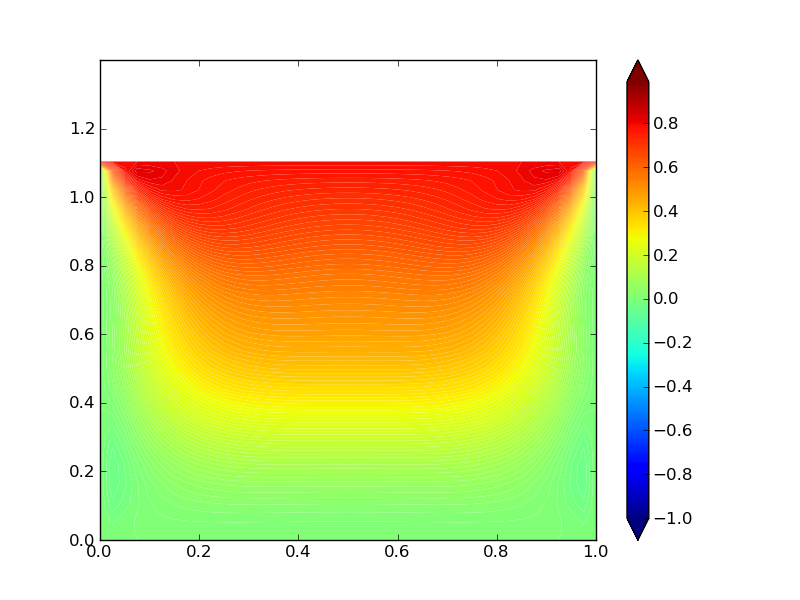
\includegraphics[width=2in]{contour-V12-ALEexp.png} \hspace{-20pt}
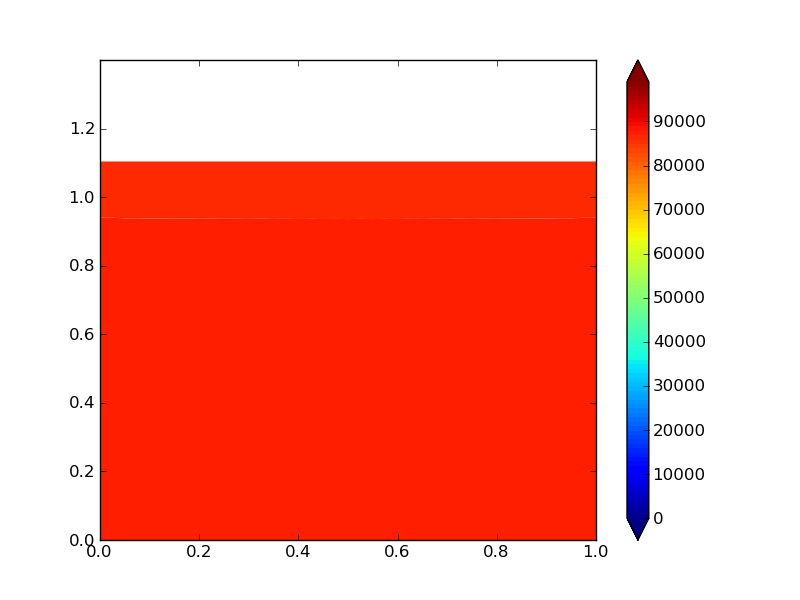
\includegraphics[width=2in]{contour-P12-ALEexp.png} \hspace{-20pt}
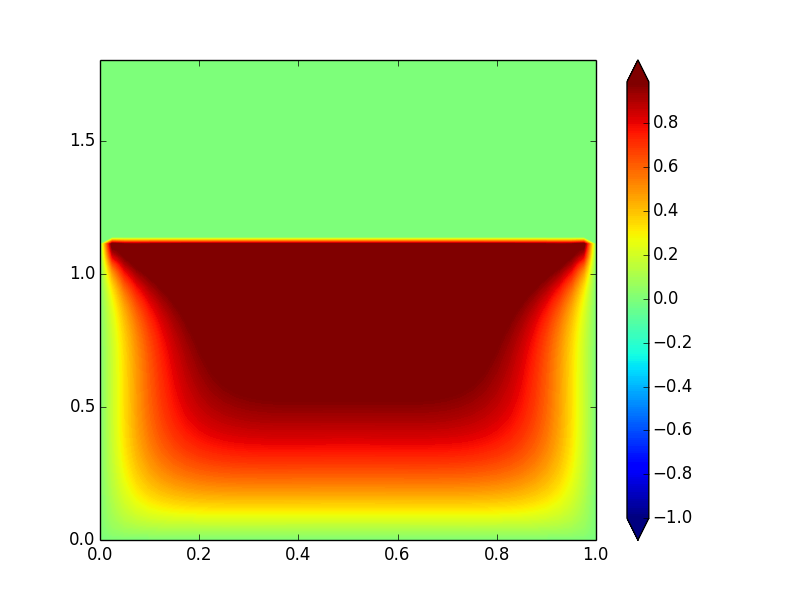
\includegraphics[width=2in]{contour-V6-IBexp.png} \hspace{-20pt}
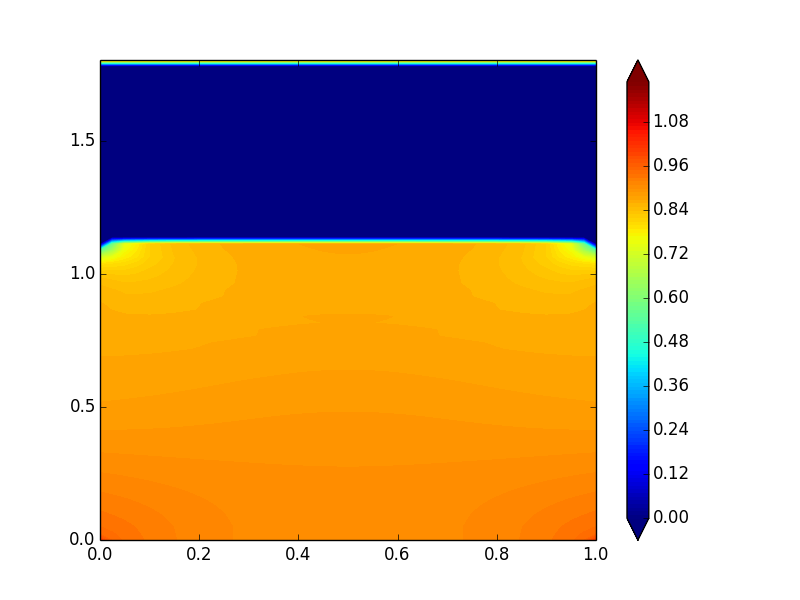
\includegraphics[width=2in]{contour-P6-IBexp.png} 
}
\vspace{-8pt}
\makebox[\textwidth][c]{\rotatebox{90}{\hspace{30pt} t$_c$ = 1/2}
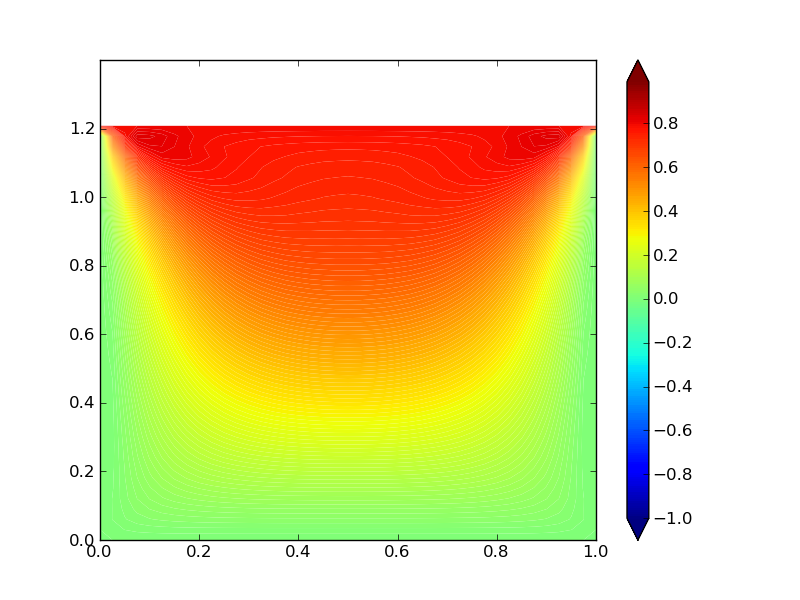
\includegraphics[width=2in]{contour-V25-ALEexp.png} \hspace{-20pt}
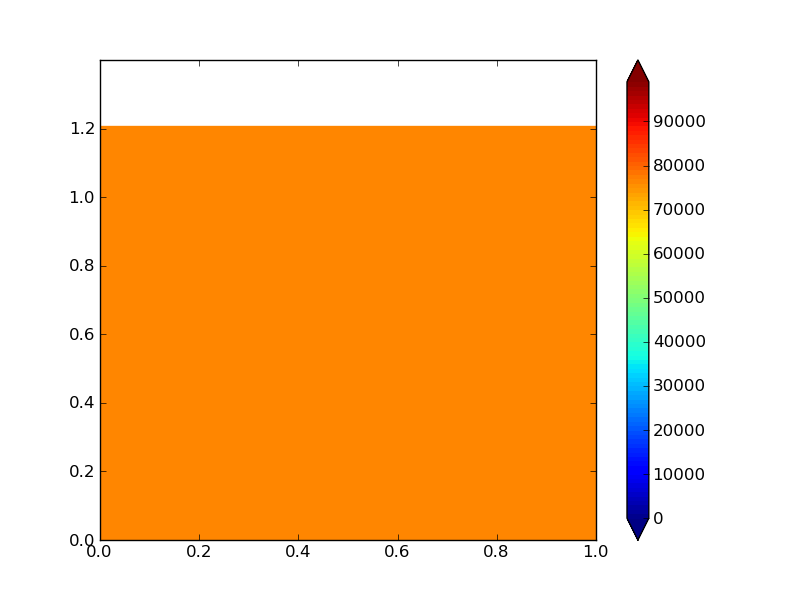
\includegraphics[width=2in]{contour-P25-ALEexp.png} \hspace{-20pt}
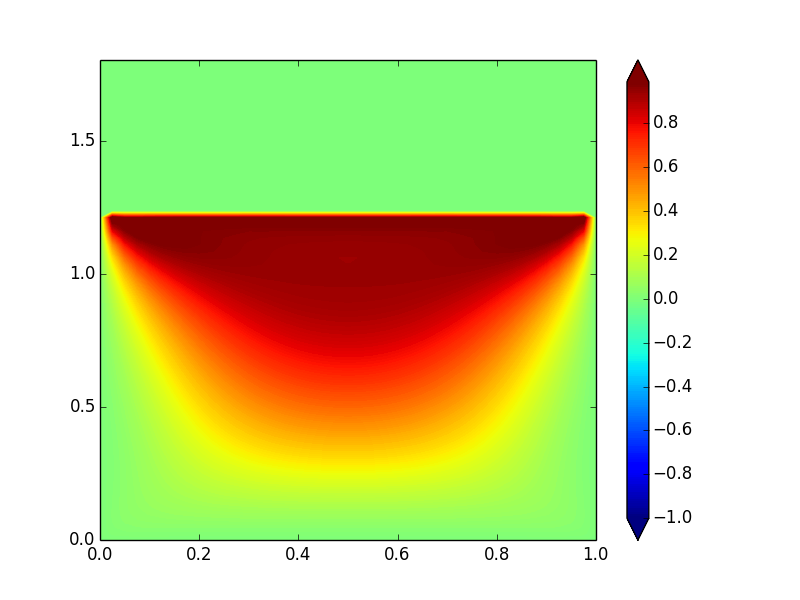
\includegraphics[width=2in]{contour-V12-IBexp.png} \hspace{-20pt}
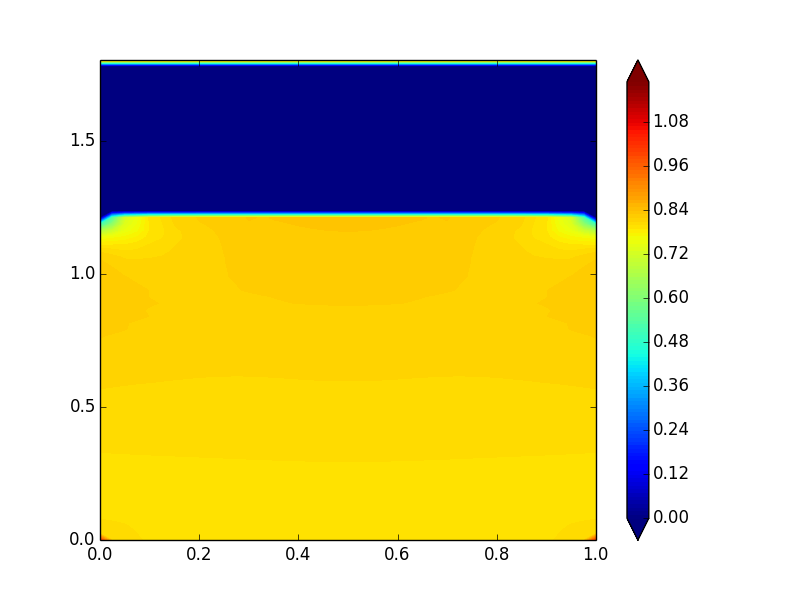
\includegraphics[width=2in]{contour-P12-IBexp.png} 
}
\vspace{-8pt}
\makebox[\textwidth][c]{\rotatebox{90}{\hspace{30pt} t$_c$ = 3/4}
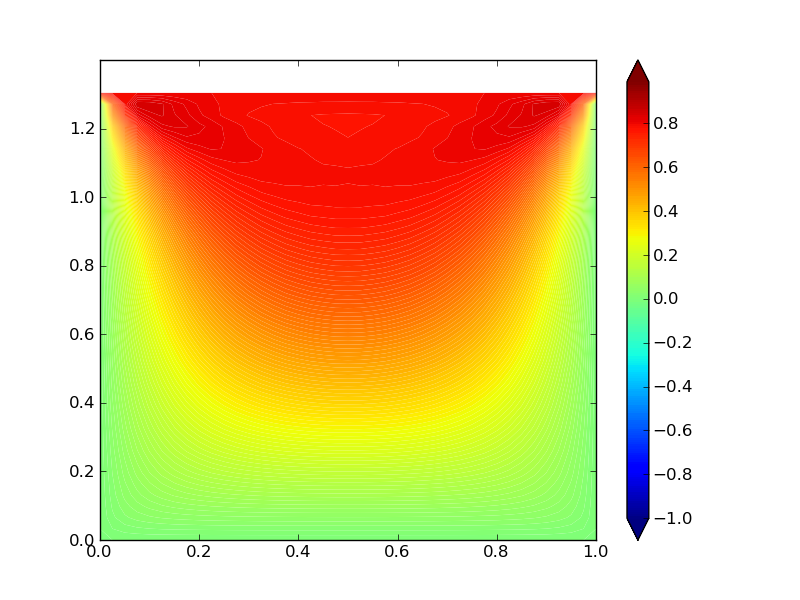
\includegraphics[width=2in]{contour-V37-ALEexp.png} \hspace{-20pt}
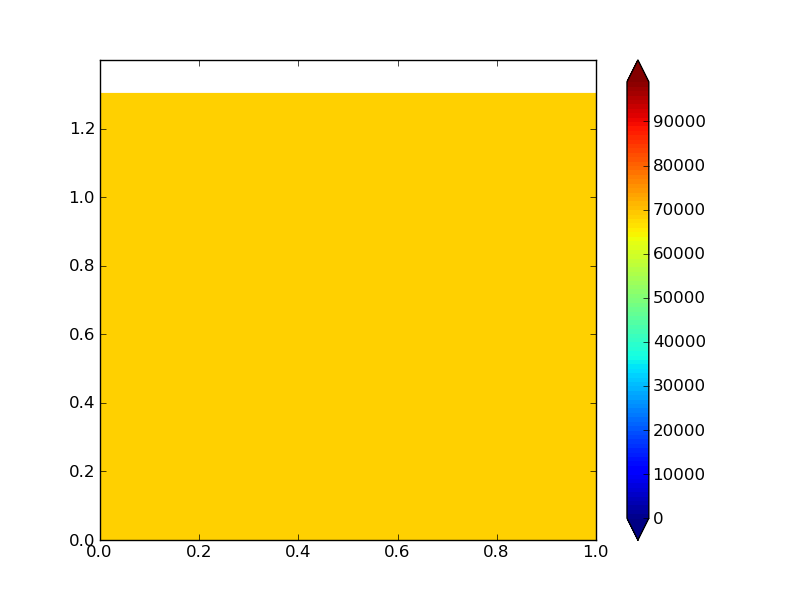
\includegraphics[width=2in]{contour-P37-ALEexp.png} \hspace{-20pt}
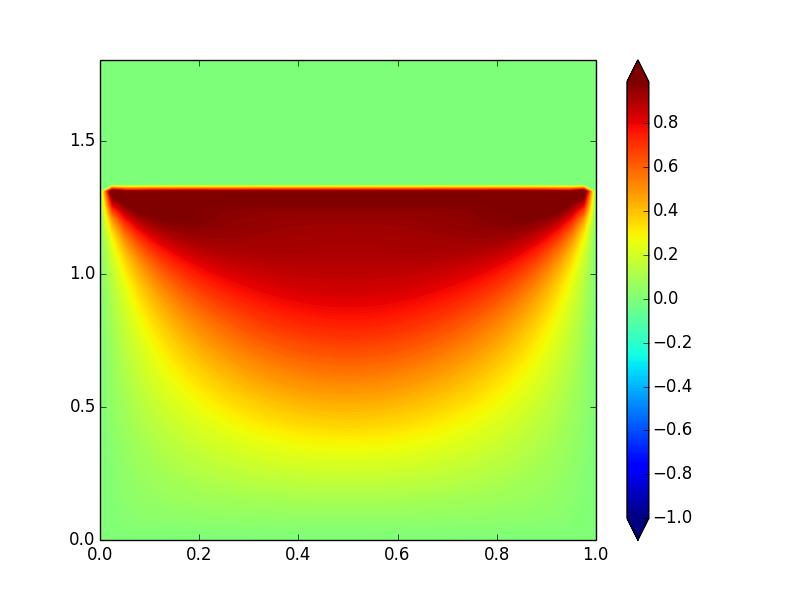
\includegraphics[width=2in]{contour-V18-IBexp.png} \hspace{-20pt}
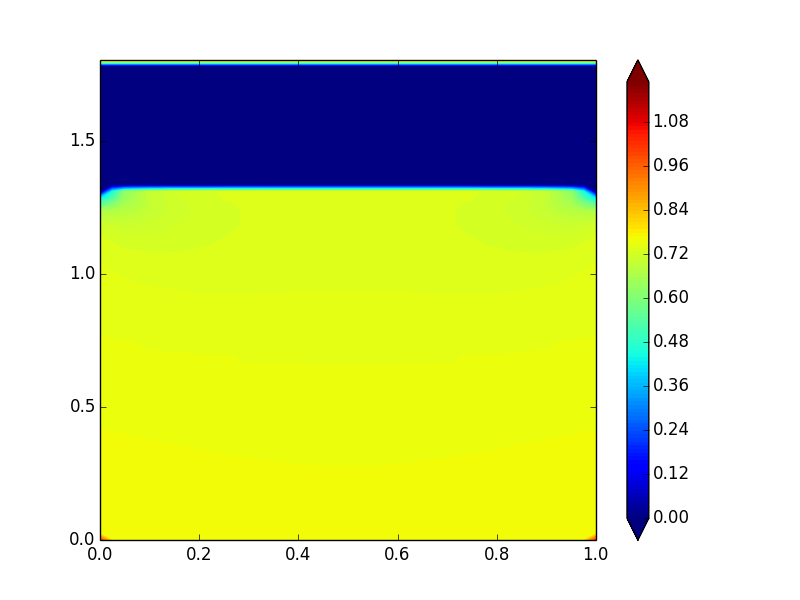
\includegraphics[width=2in]{contour-P18-IBexp.png} 
}
\vspace{-8pt}
\makebox[\textwidth][c]{\rotatebox{90}{\hspace{30pt} t$_c$ = 1}
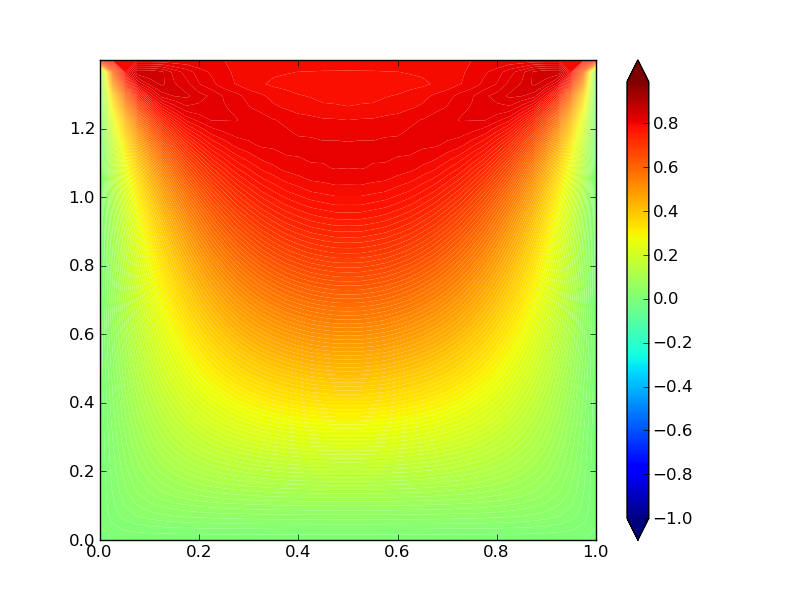
\includegraphics[width=2in]{contour-V50-ALEexp.png} \hspace{-20pt}
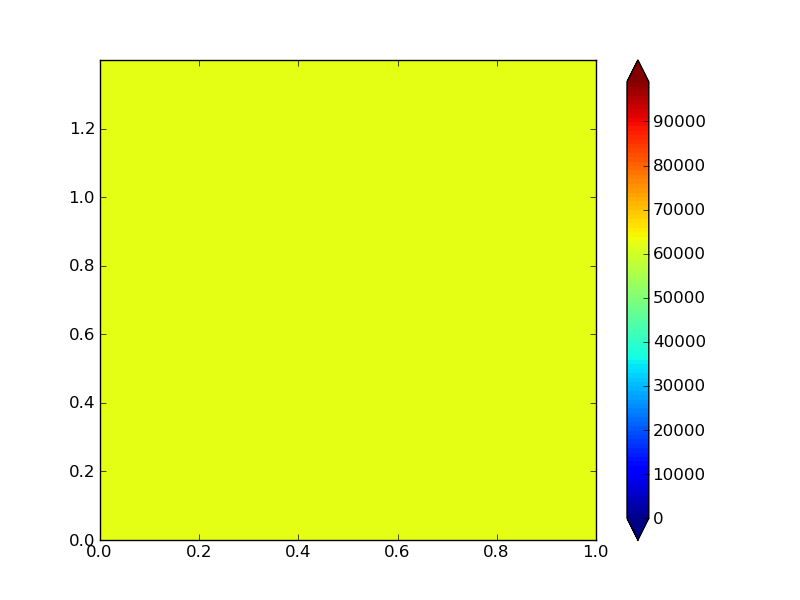
\includegraphics[width=2in]{contour-P50-ALEexp.png} \hspace{-20pt}
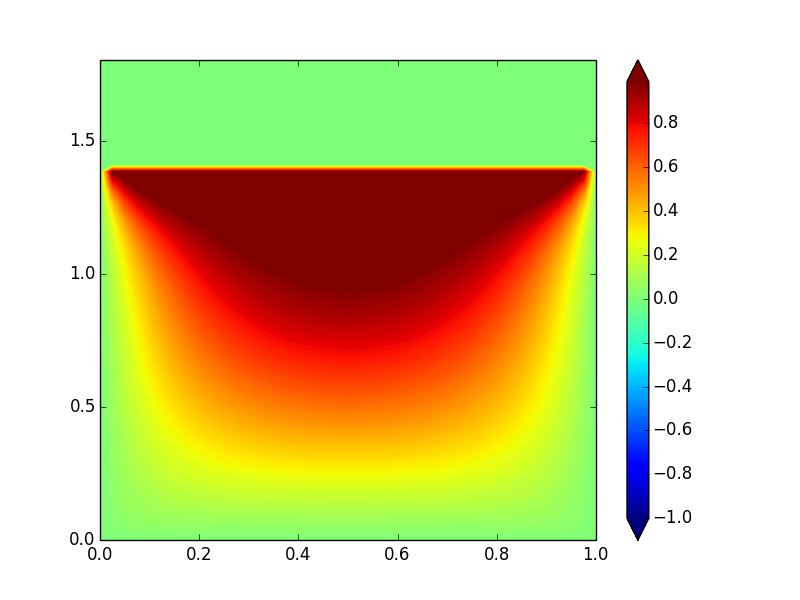
\includegraphics[width=2in]{contour-V25-IBexp.png} \hspace{-20pt}
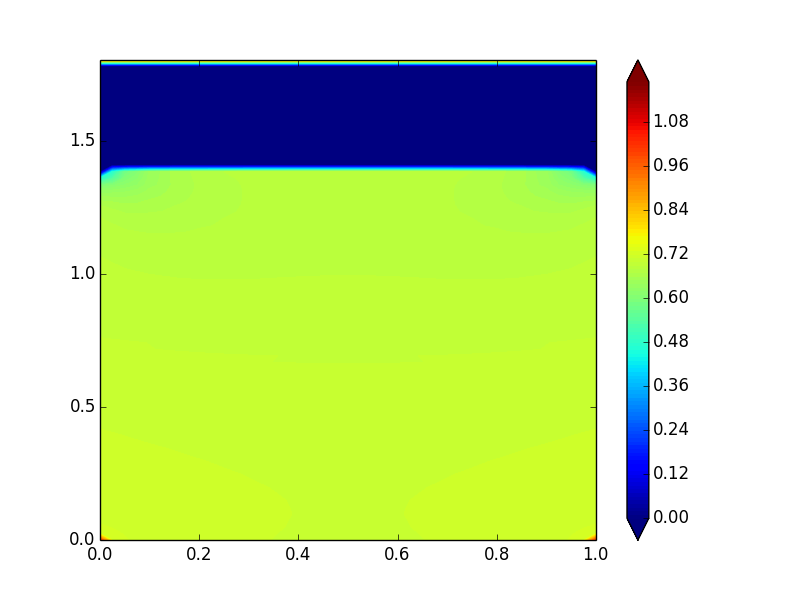
\includegraphics[width=2in]{contour-P25-IBexp.png} 
}
\caption{\label{fig:constexp} Constant velocity piston expansion for both ALE and IB methods.} 
\end{figure}
%

%
\begin{figure}
\centering
\vspace{-16pt}
\hspace{1 in} ALE \hspace{3 in} IB \\
$v$ \hspace{1.6 in} $p$\hspace{1.6 in}  $v$ \hspace{1.6 in} p
\makebox[\textwidth][c]{\rotatebox{90}{\hspace{30pt} t$_c$ = 1/4}
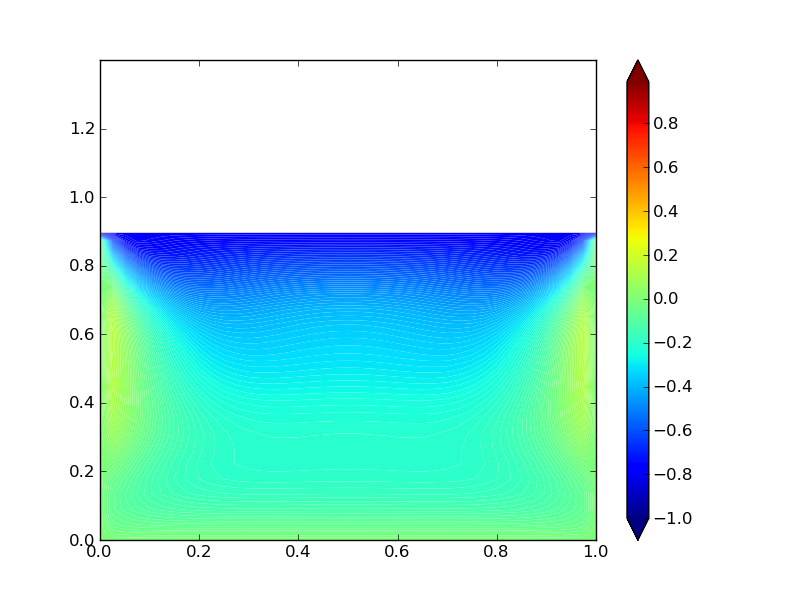
\includegraphics[width=2in]{contour-V12-ALEcomp.png} \hspace{-20pt}
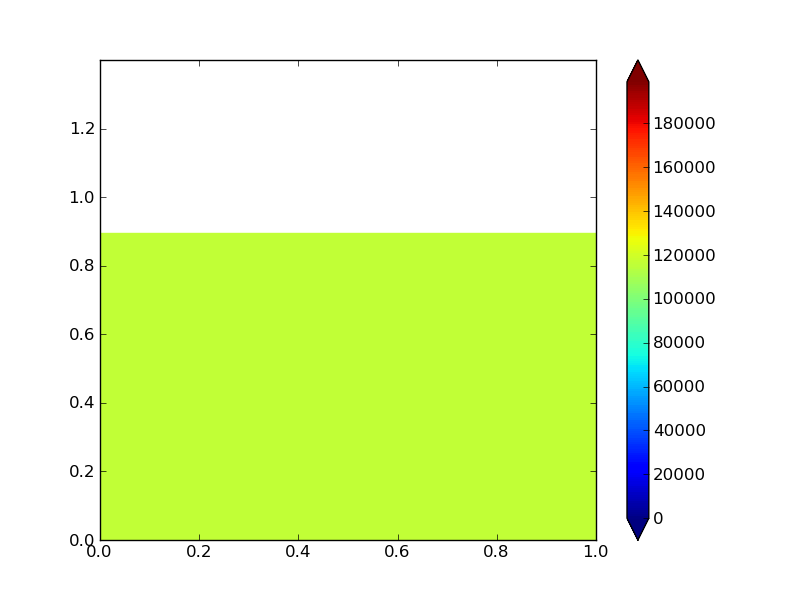
\includegraphics[width=2in]{contour-P12-ALEcomp.png} \hspace{-20pt}
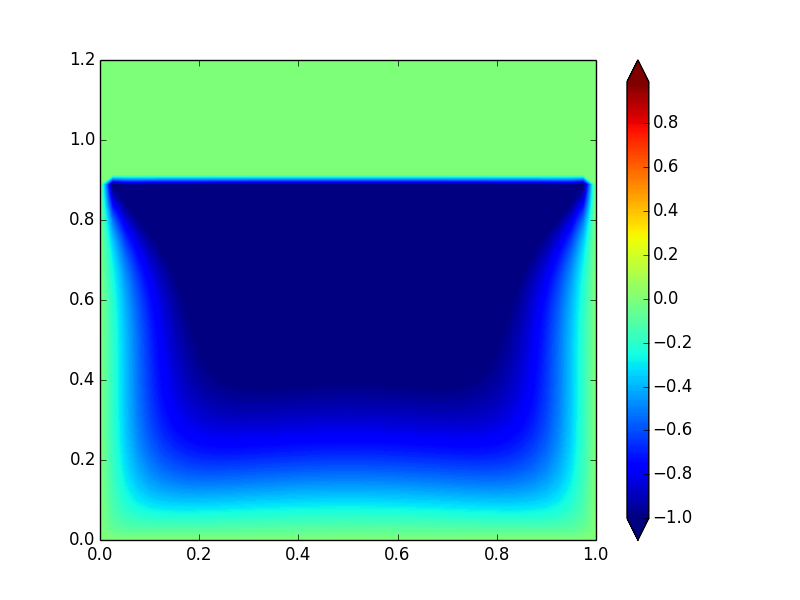
\includegraphics[width=2in]{contour-V6-IBcon.png} \hspace{-20pt}
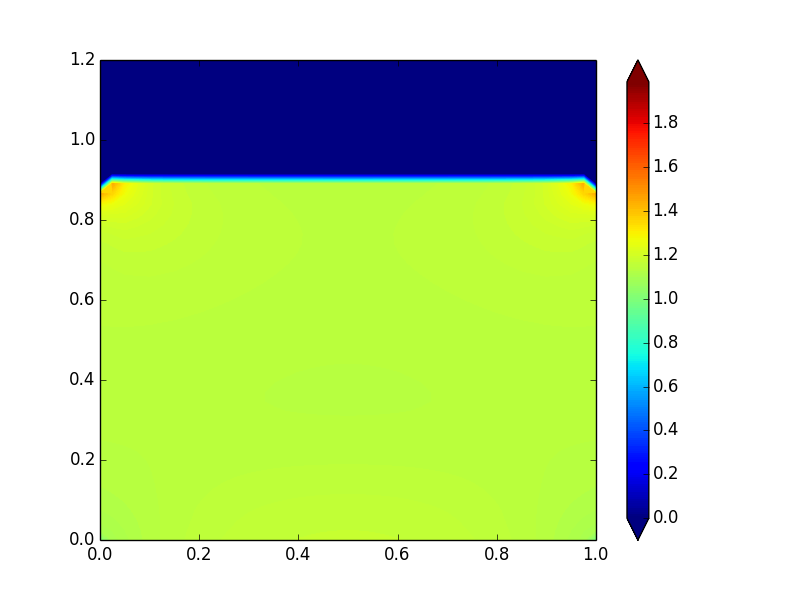
\includegraphics[width=2in]{contour-P6-IBcon.png} 
}
\vspace{-8pt}
\makebox[\textwidth][c]{\rotatebox{90}{\hspace{30pt} t$_c$ = 1/2}
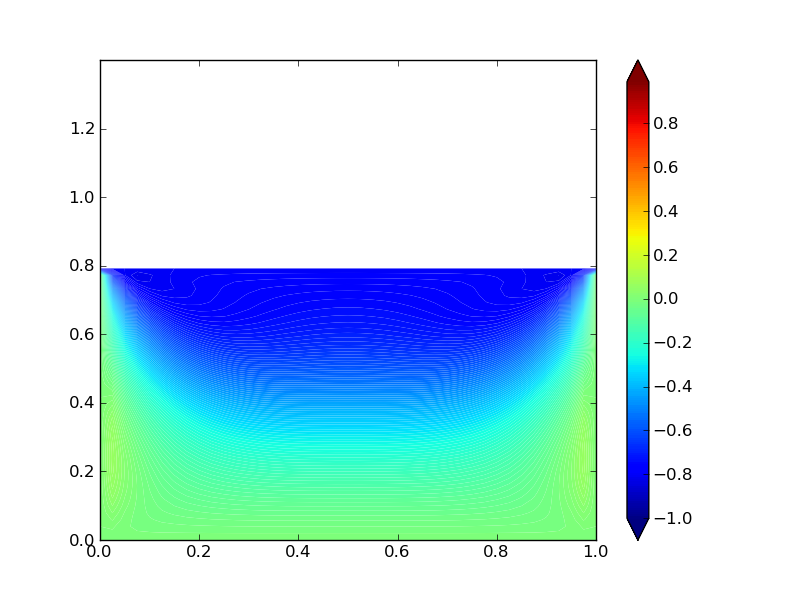
\includegraphics[width=2in]{contour-V25-ALEcomp.png} \hspace{-20pt}
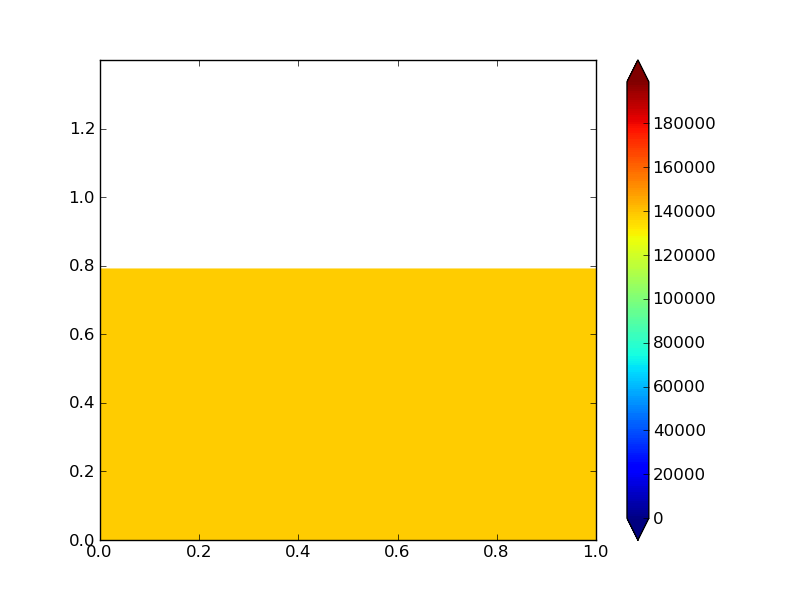
\includegraphics[width=2in]{contour-P25-ALEcomp.png} \hspace{-20pt}
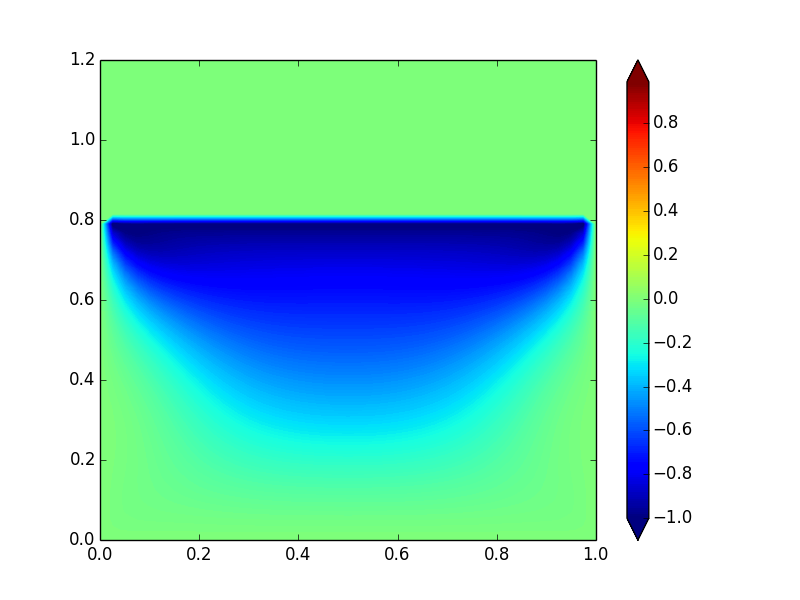
\includegraphics[width=2in]{contour-V12-IBcon.png} \hspace{-20pt}
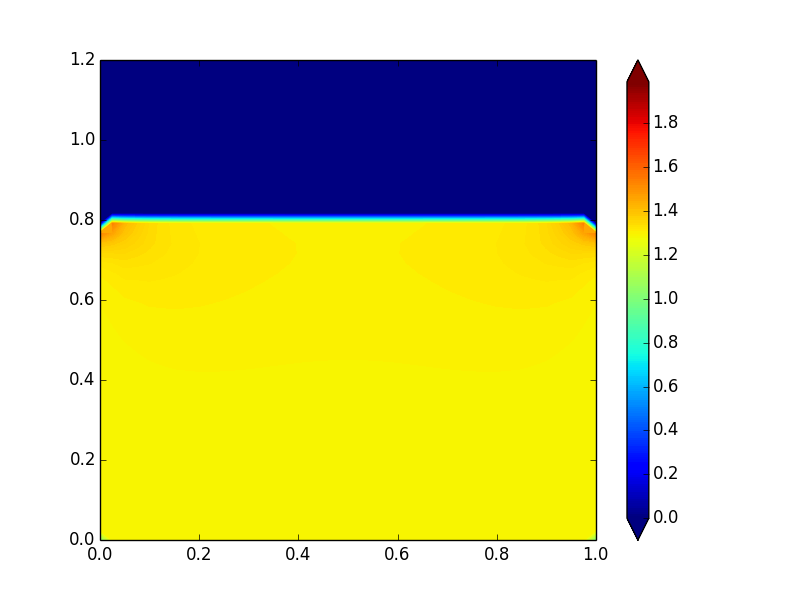
\includegraphics[width=2in]{contour-P12-IBcon.png} 
}
\vspace{-8pt}
\makebox[\textwidth][c]{\rotatebox{90}{\hspace{30pt} t$_c$ = 3/4}
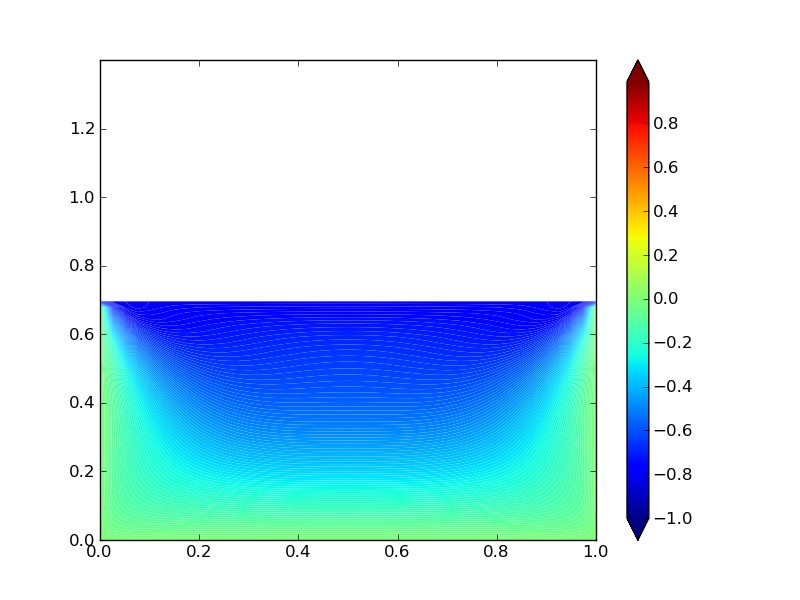
\includegraphics[width=2in]{contour-V37-ALEcomp.png} \hspace{-20pt}
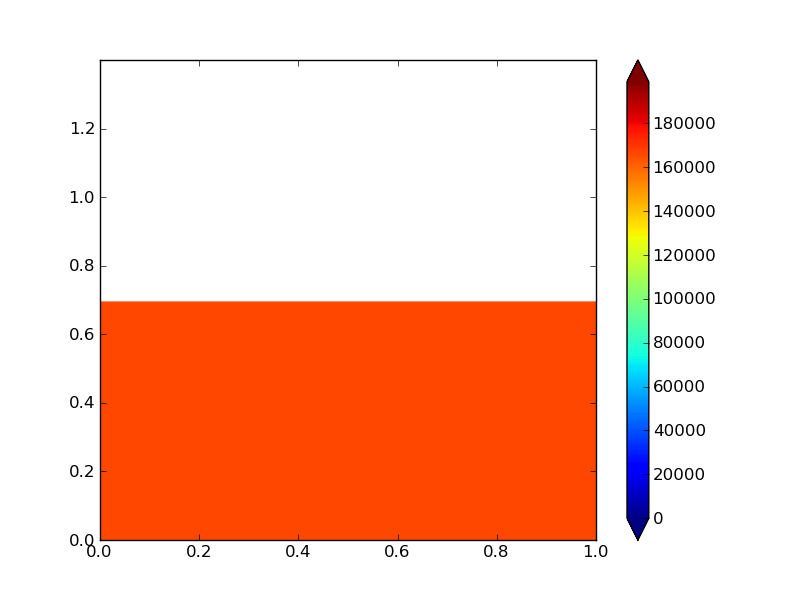
\includegraphics[width=2in]{contour-P37-ALEcomp.png} \hspace{-20pt}
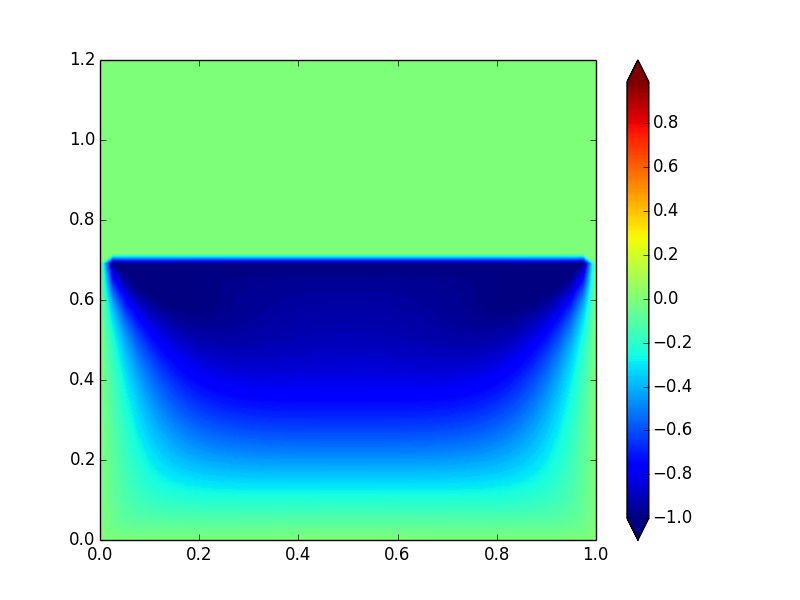
\includegraphics[width=2in]{contour-V18-IBcon.png} \hspace{-20pt}
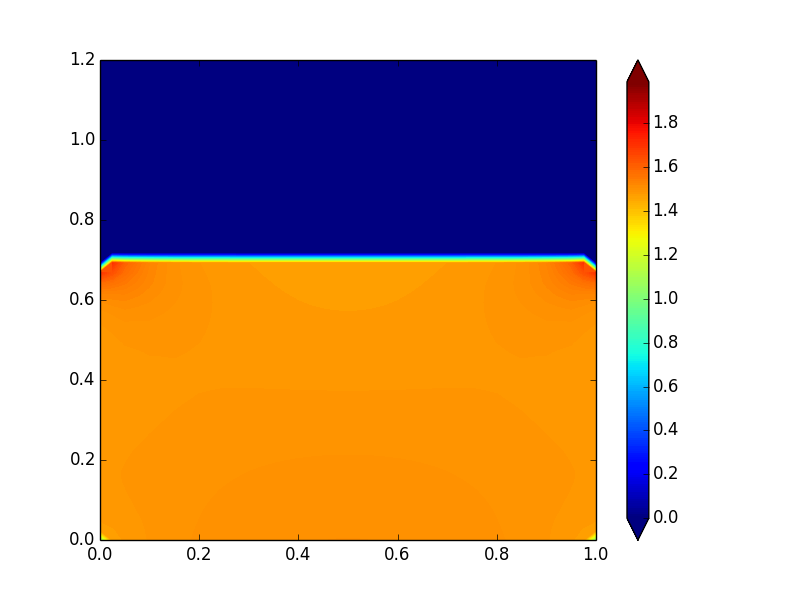
\includegraphics[width=2in]{contour-P18-IBcon.png} 
}
\vspace{-8pt}
\makebox[\textwidth][c]{\rotatebox{90}{\hspace{30pt} t$_c$ = 1}
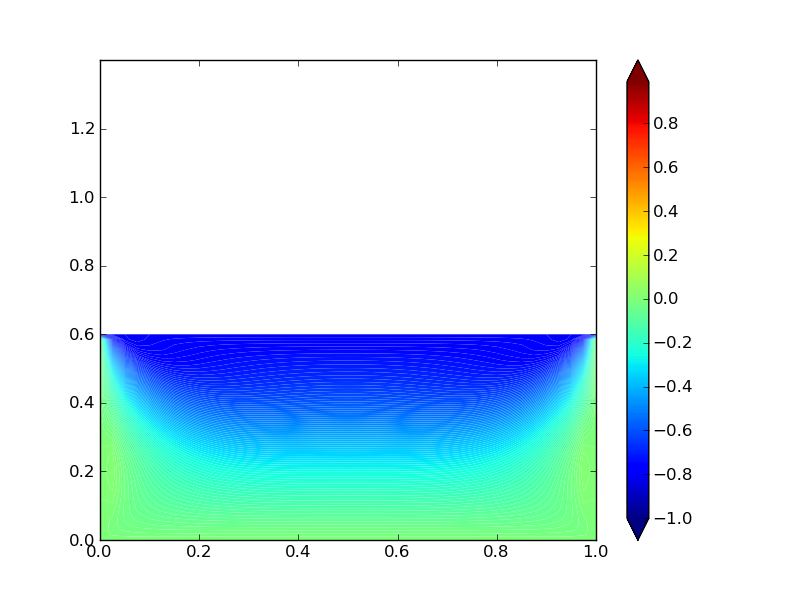
\includegraphics[width=2in]{contour-V50-ALEcomp.png} \hspace{-20pt}
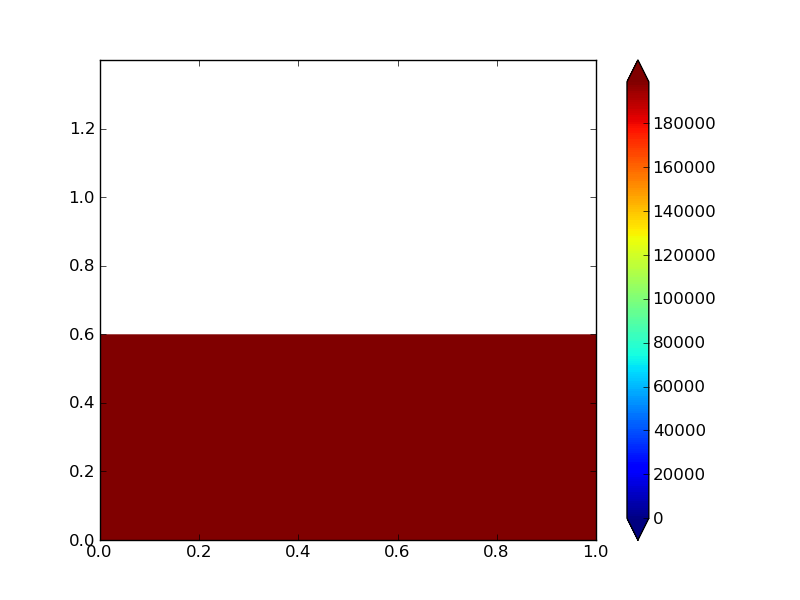
\includegraphics[width=2in]{contour-P50-ALEcomp.png} \hspace{-20pt}
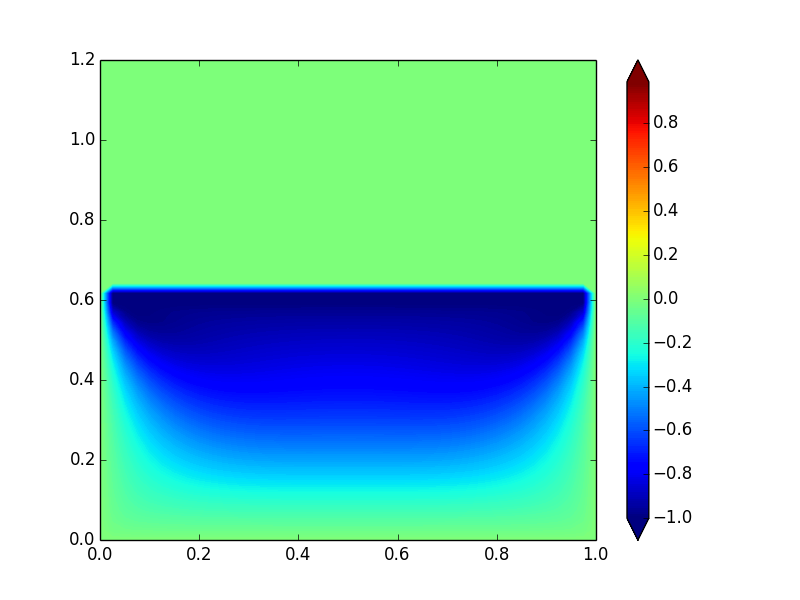
\includegraphics[width=2in]{contour-V25-IBcon.png} \hspace{-20pt}
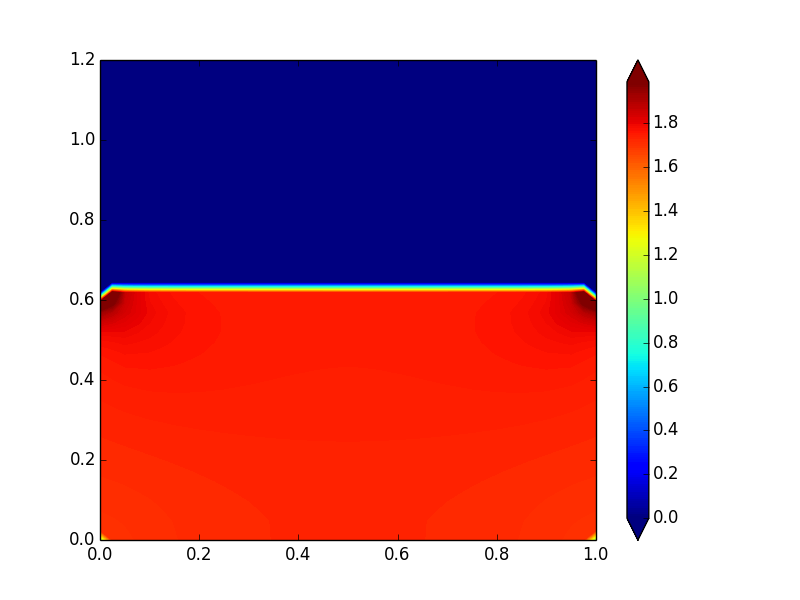
\includegraphics[width=2in]{contour-P25-IBcon.png} 
}
\caption{\label{fig:constcomp} Constant velocity piston compression for both ALE and IB methods.} 
\end{figure}
%

%
\begin{figure}
\centering
\vspace{-16pt}
\hspace{1 in} ALE \hspace{3 in} IB \\
$v$ \hspace{1.6 in} $p$\hspace{1.6 in}  $v$ \hspace{1.6 in} p
\makebox[\textwidth][c]{\rotatebox{90}{\hspace{30pt} t$_c$ = 1/4}
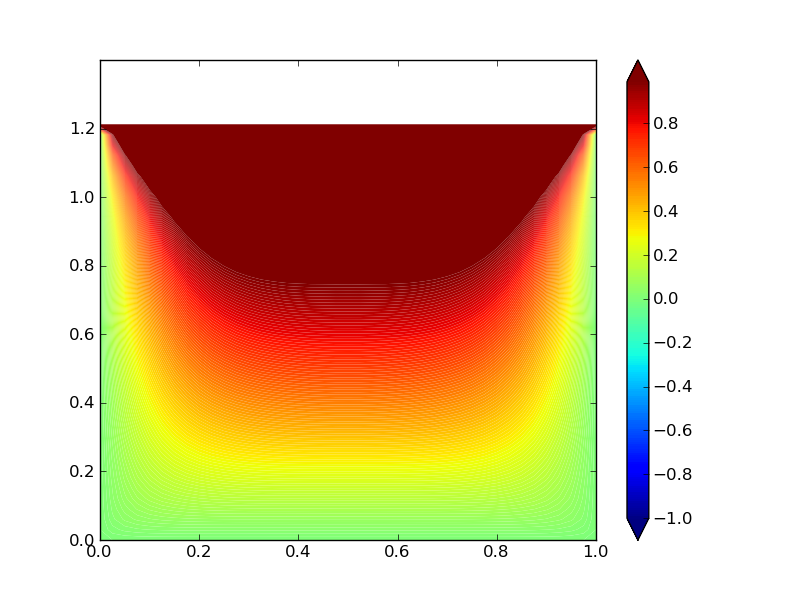
\includegraphics[width=2in]{contour-V25-ALEsin.png} \hspace{-20pt}
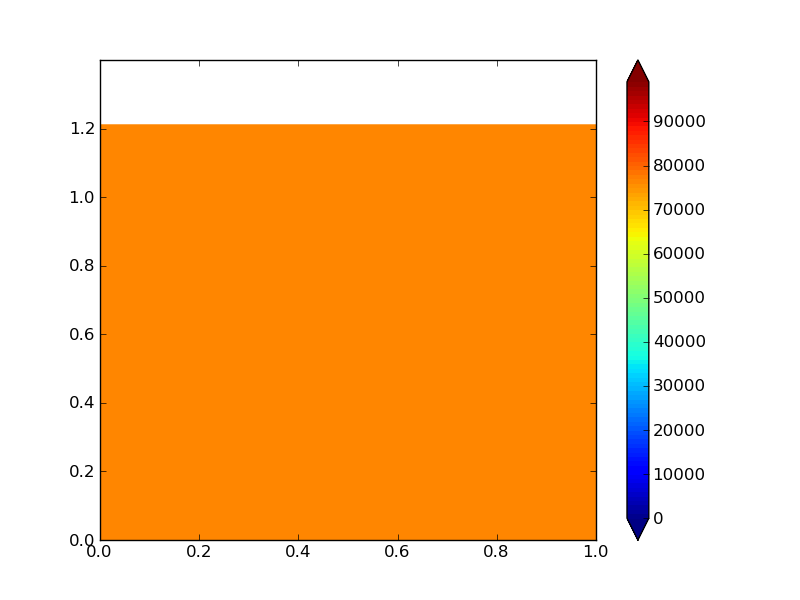
\includegraphics[width=2in]{contour-P25-ALEsin.png} \hspace{-20pt}
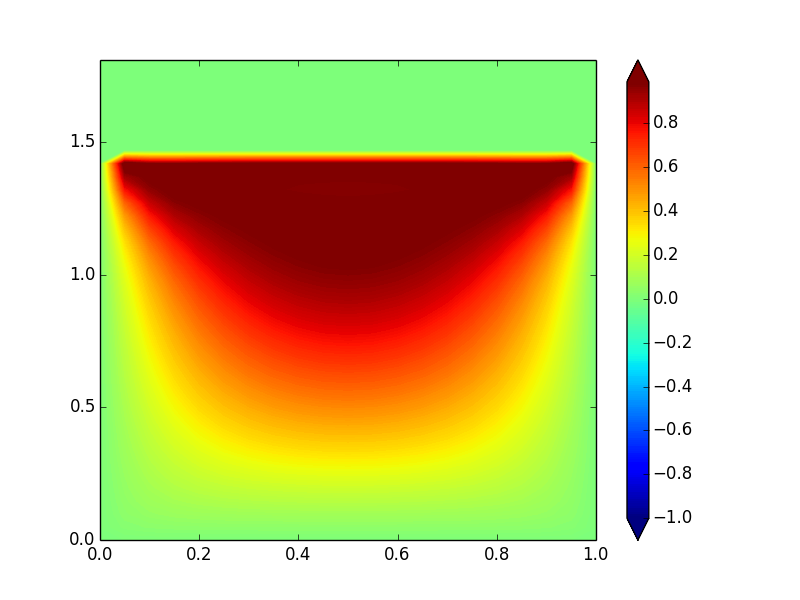
\includegraphics[width=2in]{contour-V25-IBsin.png} \hspace{-20pt}
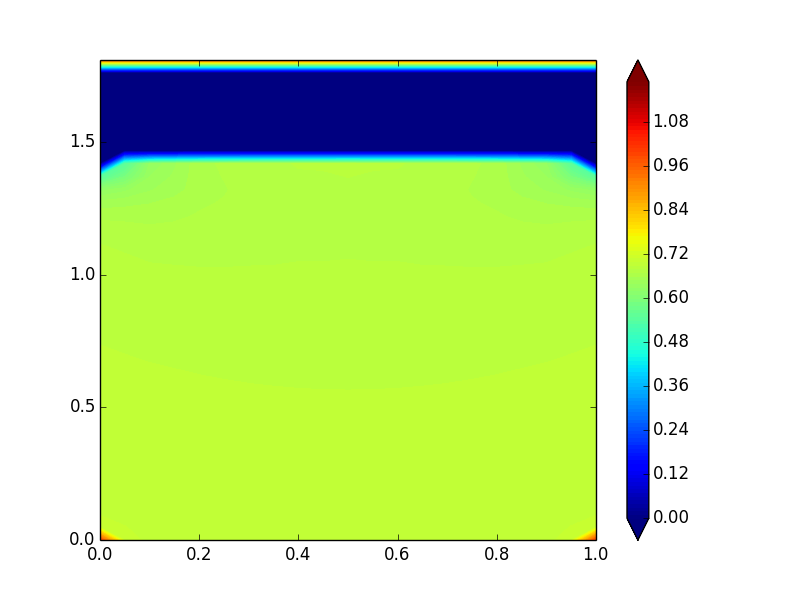
\includegraphics[width=2in]{contour-P25-IBsin.png} 
}
\vspace{-8pt}
\makebox[\textwidth][c]{\rotatebox{90}{\hspace{30pt} t$_c$ = 1/2}
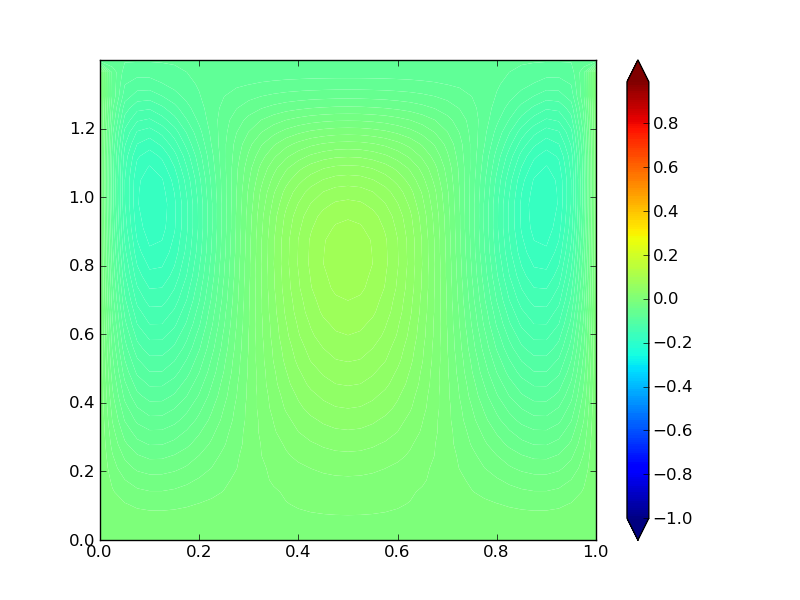
\includegraphics[width=2in]{contour-V50-ALEsin.png} \hspace{-20pt}
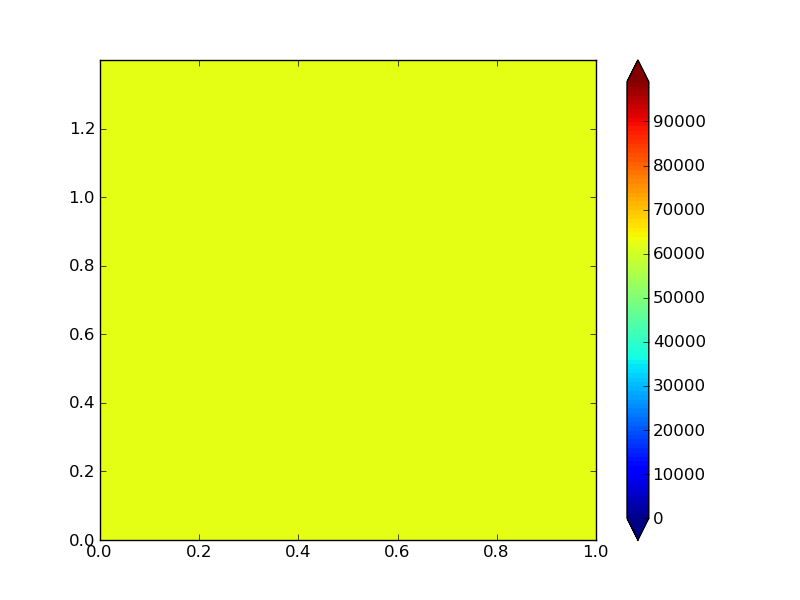
\includegraphics[width=2in]{contour-P50-ALEsin.png} \hspace{-20pt}
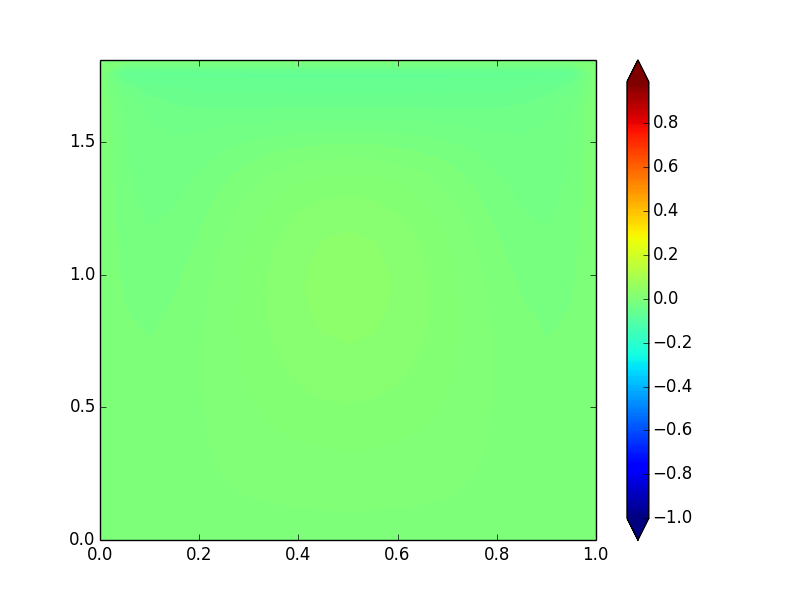
\includegraphics[width=2in]{contour-V50-IBsin.png} \hspace{-20pt}
\includegraphics[width=2in]{contour-P50-IBsin.png} 
}
\vspace{-8pt}
\makebox[\textwidth][c]{\rotatebox{90}{\hspace{30pt} t$_c$ = 3/4}
\includegraphics[width=2in]{contour-V75-ALEsin.png} \hspace{-20pt}
\includegraphics[width=2in]{contour-P75-ALEsin.png} \hspace{-20pt}
\includegraphics[width=2in]{contour-V75-IBsin.png} \hspace{-20pt}
\includegraphics[width=2in]{contour-P75-IBsin.png} 
}
\vspace{-8pt}
\makebox[\textwidth][c]{\rotatebox{90}{\hspace{30pt} t$_c$ = 1}
\includegraphics[width=2in]{contour-V100-ALEsin.png} \hspace{-20pt}
\includegraphics[width=2in]{contour-P100-ALEsin.png} \hspace{-20pt}
\includegraphics[width=2in]{contour-V100-IBsin.png} \hspace{-20pt}
\includegraphics[width=2in]{contour-P100-IBsin.png} 
}
\caption{\label{fig:sinusoid} Sinusoidal velocity piston expansion and compression for both ALE and IB methods.} 
\end{figure}
%

\subsection{Immersed Boundary}

The general trends observed using the immersed boundary method are quite similar to those for ALE, as shown in Figures \ref{fig:constexp}, \ref{fig:constcomp}, and \ref{fig:sinusoid}. For the expansion, as epxected, the pressure in the chamber decreases and the velocity behind the piston increases to match the piston velocity. Due to the low Reynolds numer of the test cases, significant dissipation occurs near the walls, resulting in an almost parabolic velocity distribution in the region behind the piston. The observed behavior for the piston advancement is similar, although reversed. Pressure increases and the flow is pushed toward the bottom wall of the piston. There are some spurious pressure overpredictions near the corners of the piston head in this case, which indicates that the immersed boundary method may become inacurate near high gradient regions, such as corners. Lastly, for the sinusoidal case similar trends are again observed. The only notable difference between the two cases is that at $t_c = 1/2$ and $t_c = 1$, when the piston is at the point of its sycle where it is instantaneously stopped, the ALE method predicts some lingering fluid motion, while the IB method predicts no motion. This may be a result of slight differences in conditions between the two methods. 

\subsection{Effect of Ma and Re}

The effects of varying Reynolds number at constant Mach number and varying Mach number at constant Reynolds number are shown in Figure \ref{fig:parameters}. Comparing the top left grouping to the bottom left grouping, it can be seen that at low Reynlds numbers, viscous damping near the walls significantly slows the flow near the walls, chsanging the shape of the velocity profiles and leading to a more diffuse transition between the moving and non-moving regions. For the high Re case, pressure waves propogate back and forth, reflecting off of the bottom wall and the moving piston. However, for the low Re case, the waves are damped out by viscous effects. 

The Mach number also plays a significant role in the form of the solution. For the comparison between the top left grouping and top right grouping of Figure \ref{fig:parameters}, the piston velocity and Reynolds number are held constant while the Mach number is increased from 0.1 to 0.8. Effectively, the relaive propagation speed of pressure waves is reduced for the Ma= 0.8 case. As stated previously, for the low Mach number case pressure waves are much faster than the piston motion, and therefore have time to reflect off the solid bottom boundary several times. Each reflection further increases the pressure in the chamber. However, for the Ma = 0.8 case, the pressure wave propogates only slightly faster than the piston motion, leading to a high pressure region adjacent to the piston, with a sharp transition to a low pressure region away from the piston. Overall, the trends observed here agree qith physical expectations, providing further support to methods utlized have been correctly implemented.

%
\begin{figure}
\centering
\vspace{-16pt}
\hspace{0.5 in} Ma = 0.1, Re = 100 \hspace{2.5 in} Ma = 0.8, Re = 100 \\
$v$ \hspace{1.6 in} $p$\hspace{1.6 in}  $v$ \hspace{1.6 in} p
\makebox[\textwidth][c]{\rotatebox{90}{\hspace{30pt} t$_c$ = 1/2}
\includegraphics[width=2in]{contour-V12-re100.png} \hspace{-20pt}
\includegraphics[width=2in]{contour-P12-re100.png} \hspace{-20pt}
\includegraphics[width=2in]{contour-V12-ma08.png} \hspace{-20pt}
\includegraphics[width=2in]{contour-P12-ma08.png} 
}
\vspace{-8pt}
\makebox[\textwidth][c]{\rotatebox{90}{\hspace{30pt} t$_c$ = 1}
\includegraphics[width=2in]{contour-V25-re100.png} \hspace{-20pt}
\includegraphics[width=2in]{contour-P25-re100.png} \hspace{-20pt}
\includegraphics[width=2in]{contour-V25-ma08.png} \hspace{-20pt}
\includegraphics[width=2in]{contour-P25-ma08.png} 
}
\vspace{0pt}\\
\hspace{-3 in} Ma = 0.1, Re = 5 \\
\vspace{0pt}
\makebox[\textwidth][c]{\rotatebox{90}{\hspace{30pt} t$_c$ = 1/2}
\includegraphics[width=2in]{contour-V12-IBcon.png} \hspace{-20pt}
\includegraphics[width=2in]{contour-P12-IBcon.png} \hspace{260pt}
}
\vspace{-8pt}
\makebox[\textwidth][c]{\rotatebox{90}{\hspace{30pt} t$_c$ = 1}
\includegraphics[width=2in]{contour-V25-IBcon.png} \hspace{-20pt}
\includegraphics[width=2in]{contour-P25-IBcon.png} \hspace{260pt} 
}
\caption{\label{fig:parameters} Comparison of constant velocity piston advancement (compression) for different flow parameters.} 
\end{figure}
%


%----------------------------------------------------------------------------------------
%	SECTION 5
%----------------------------------------------------------------------------------------

\section{Conclusions}

In this work, we have presented two methods for solving a problem with moving boundaries.  The ALE method solves the issue of the moving boundary by advecting the grid at a velocity between the speed of the flow and zero, and solves the equations in this frame.  The IB method uses additional cells and a forcing function to enforce the moving boundary on the larger grid.  The two methods have been used on a two dimensional piston problem with comparable boundary conditions.  The two methods yield similar results; however, the overall performance of the IB method is significantly better over a wider range of conditions, as the ALE method appears to have numerical stability issues.  Additionally, the IB method is easier to implement in a code architecture which does not already possess moving grids, and avoids the difficult business of determining propagation and remeshing in situations where more complex boundary geometries are present.


%----------------------------------------------------------------------------------------
%	BIBLIOGRAPHY
%----------------------------------------------------------------------------------------

\bibliographystyle{plain}

\bibliography{finproj}

%----------------------------------------------------------------------------------------


\end{document}
